\chapter{OpenCAL}\label{ch:opencal}

This Chapter introduces the serial implementation of OpenCAL by
examples. After a brief overview about supported data, main structure
and adopted conventions, the implementation of a simple 2D CA is described. Subsequently, four different
implementations of a more complex 2D example are illustrated, to show
how simulation efficiency can be improved. The implementation of a
simple 3D CA is also presented for the sake of completeness. The last
part of the Chapter deals with OpenCAL-GL and shows how to integrate a
basic OpenGL/GLUT visualization system in both 2D and 3D OpenCAL-based
applications.


\section{Basic data types and main loop structure}

The current version of OpenCAL provides support for three different
basic scalar types and substates, besides CA and simulation
objects. Supported scalar types and substates are listed in Table
\ref{tab:basic_types} and \ref{tab:substate_types}, respectively,
while Table \ref{tab:ca_sim_types} lists CA and simulation data types.

\begin{table}
  \centering
  \begin{tabular}{c|c|c}
    \hline
    OpenCAL basic type & Parameters alias & Corresponding C type \\
    \hline
    \verb'CALbyte' & \verb'CALParameterb' & \verb'char'  \\
    \verb'CALint'  & \verb'CALParameteri' & \verb'int'  \\
    \verb'CALreal' & \verb'CALParameterr' & \verb'double'  \\
    \hline
  \end{tabular}
  \caption{OpenCAL basic types, together with their alias, used for
    defining CA parameters, and correspondent types in C.}
  \label{tab:basic_types}
\end{table}

\begin{table}
  \centering
  \begin{tabular}{l|l}
    \hline
    OpenCAL substate type & Basic scalar type \\
    \hline
    \verb'CALSubstate[2D|3D]b' & \verb'CALbyte'\\
    \verb'CALSubstate[2D|3D]i' & \verb'CALint' \\
    \verb'CALSubstate[2D|3D]r' & \verb'CALreal'\\
    \hline
  \end{tabular}
  \caption{OpenCAL substate types, together with their basic scalar
    types.}
  \label{tab:substate_types}
\end{table}

\begin{table}
  \centering
  \begin{tabular}{l|l}
    \hline
    OpenCAL substate type & Meaning \\
    \hline
    \verb'CALModel[2D|3D]' & CA data type\\
    \verb'CALRun2D[2D|3D]' & Simulation data type\\
    \hline
  \end{tabular}
  \caption{OpenCAL types for CA and simulation objects.}
  \label{tab:ca_sim_types}
\end{table}


Figure \ref{fig:opencal_main_loop} shows the OpenCAL main simulation
loop. Before entering the loop, if defined, the init function is
executed once and a substates update performed. Afterwards, while the
current step is lower or equal to the final step of computation (or
this latter is set to \verb'CAL_RUN_LOOP', which defines an infinite
loop), elementary processes are executed once at a time, in the order
they have been registered to the CA. Here, note that a substates
update is performed after each elementary process. Moreover, just
before the end of the computational step, the steering function (if
defined) is applied and a substates update performed. At the end of
the computational step, a stop condition is checked, which can stop
the simulation even before the last step is reached.


\begin{figure}[htbp]
  \centering
  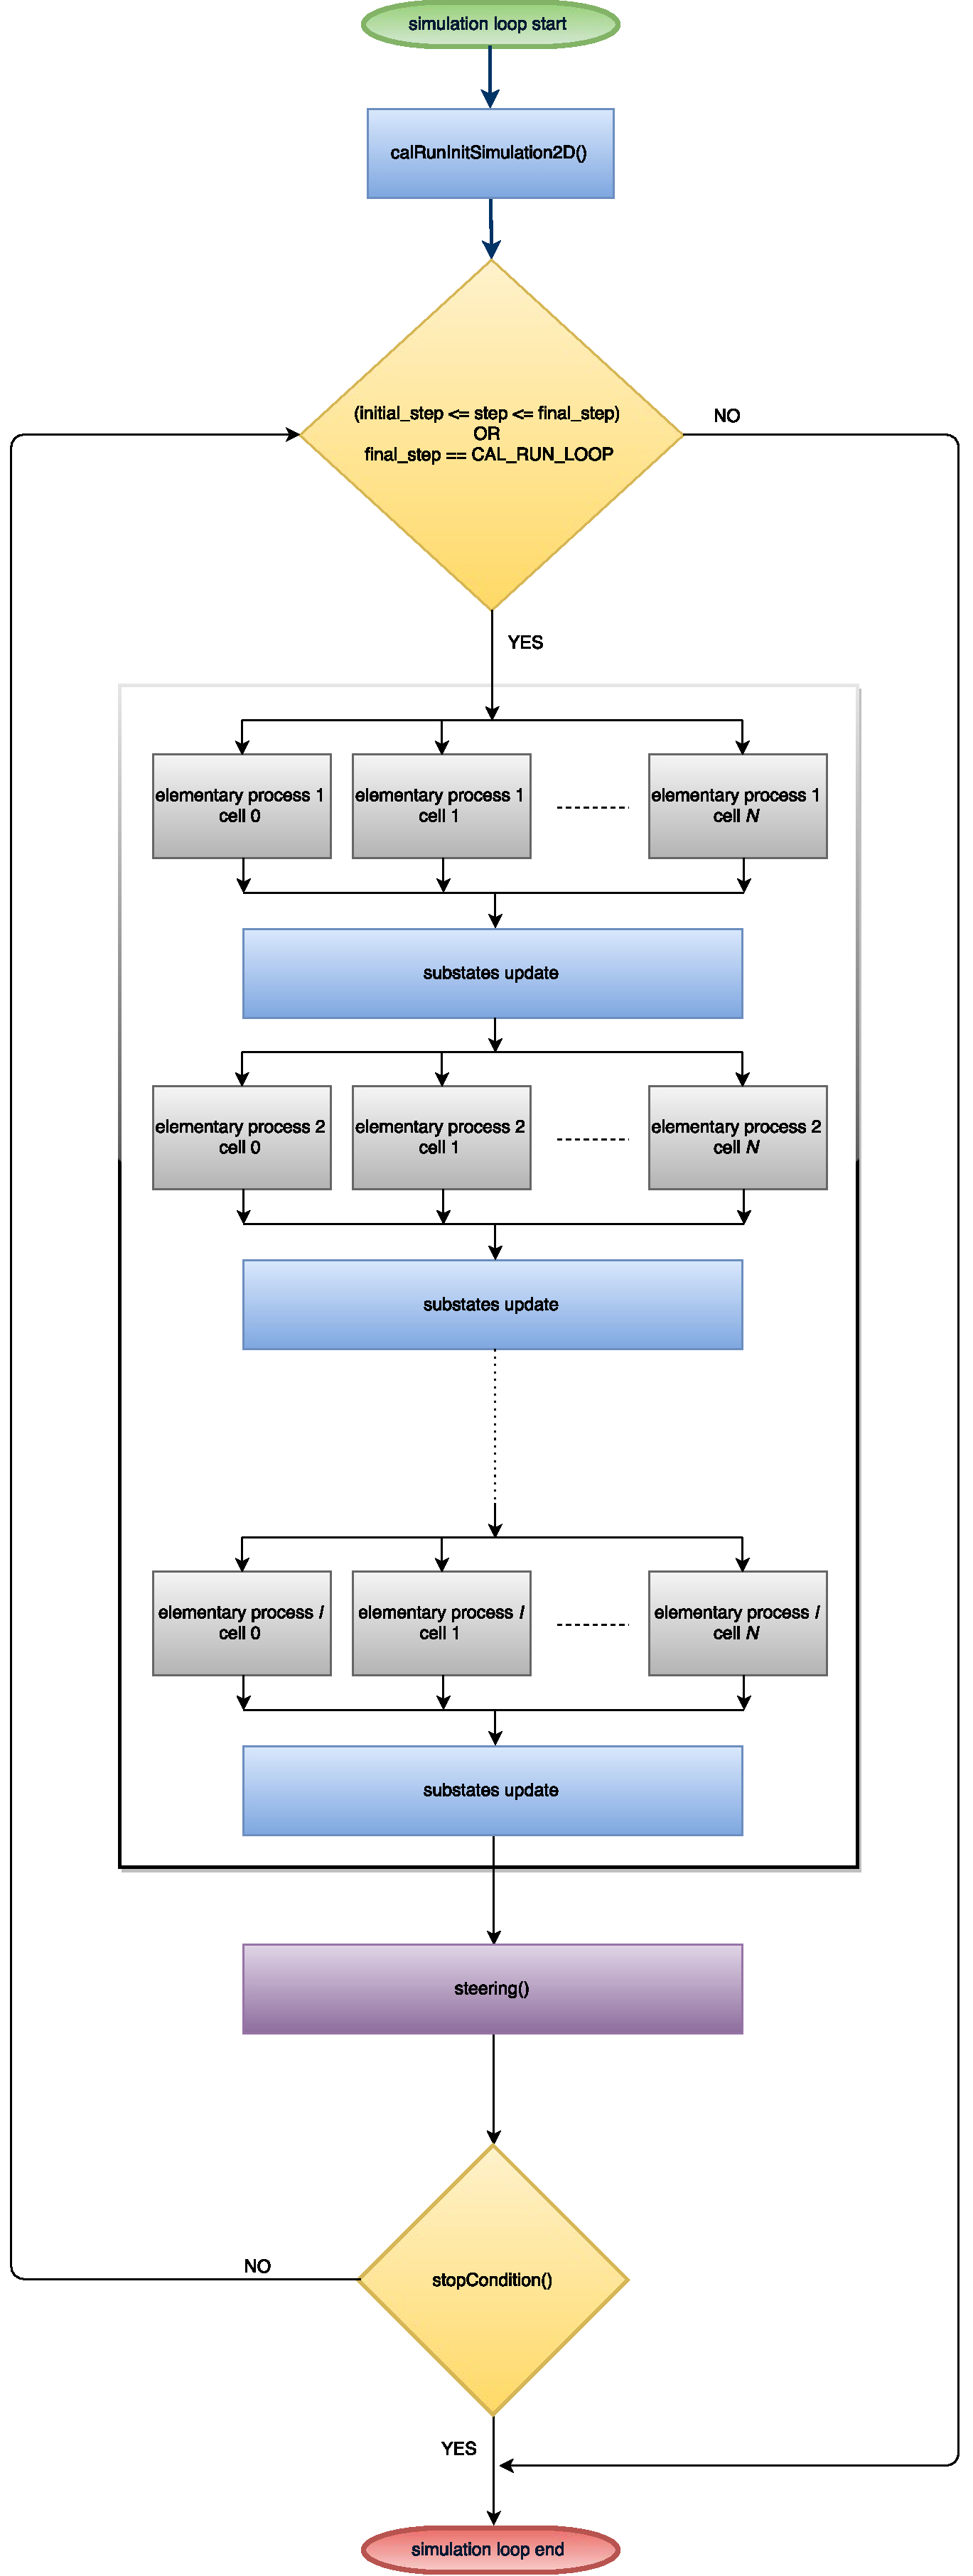
\includegraphics[width=9.5cm]{./images/OpenCAL/opencal_main_loop.pdf}
  \caption{OpenCAL main loop chart.}
  \label{fig:opencal_main_loop}
\end{figure}


\section{Statements conventions}\label{sec:Conventions}

As seen, data types have the same \verb'CAL' prefix, and an
optional suffix identifying the CA dimension or the basic scalar type,
or both of them. For instance, the 2Di suffix specifies a
two-dimensional object in which each element is of type integer
(cf. Table \ref{tab:substate_types}).

Predefined numerical constants start with the \verb'CAL_' prefix,
followed by at least one uppercase keyword. In case of more keywords,
they are separated by the \verb'_' character.

Eventually, functions start with the \verb'cal' suffix, followed by at
least one capitalized keyword, and end with a suffix specifying the CA
dimension and the basic datatype.


\section{Conway's Game of Life}\label{sec:cal_life}

In order to introduce OpenCAL, this section starts by implementing the
Conway's Game of Life, one of the most simple, yet powerful examples
of CA, devised by mathematician John Horton Conway in 1970.

The Game of Life can be thought as an infinite two-dimensional
orthogonal grid of square cells, each of which is in one of two
possible states, \emph{dead} or \emph{alive}. Every cell interacts
with the eight adjacent neighbors belonging to the Moore
neighborhood. At each time step, one of the following transitions
occur:

\begin{enumerate}
    \item Any live cell with fewer than two alive neighbors dies, as
      if by loneliness.
    \item Any live cell with more than three alive neighbors dies, as
      if by overcrowding.
    \item Any live cell with two or three alive neighbors lives,
      unchanged, to the next generation.
    \item Any dead cell with exactly three live neighbors comes to
      life.
\end{enumerate}

The initial configuration of the system specifies the state (dead or
alive) of each cell in the cellular space. The evolution of the
system is thus obtained by applying the above rules (which define the
cell's transition function) simultaneously to every cell in the
cellular space, so that each new configuration is function of the one
at the previous step. The rules continue to be applied repeatedly to
create further generations. For more details on the Game of Life,
please check Wikipedia at the URL
\url{http://en.wikipedia.org/wiki/Conway's_Game_of_Life}.

\begin{figure}
  \begin{center}
    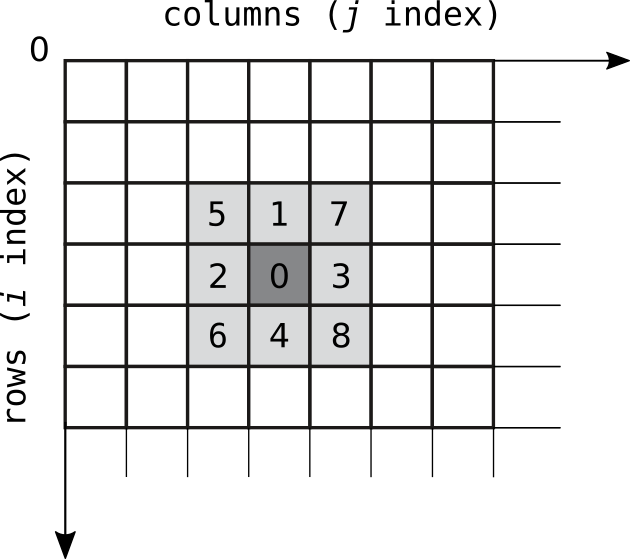
\includegraphics[width=5cm]{./images/OpenCAL/LifeNeighborhood.png}
    \caption{OpenCAL's 2D cellular space and Moore neighborhood. Cells
      are individuated by a couple of matrix-style integer coordinates
      $(i, j)$, where $i$ represents the row and $j$ the column. Cell
      (0,0) is the one located at the upper-left corner. Moore
      neighborhood is represented in gray, with the central cell
      highlighted in dark gray. Neighboring cells can also be indexed by
      the integer subscripts shown within the cells. Cells indices are
      implicitly assigned by OpenCAL, both in the case of predefined
      and custom neighborhoods. In the first case, indices can not be
      modified, while in the second case, indices are assigned
      progressively in an automatic way each time a new neighbor is added
      to the CA by means of the \texttt{calAddNeighbor2D()} function.}
    \label{fig:LifeNeighborhood}
  \end{center}
\end{figure}

The formal definition of the Life CA is reported below.

$$Life = < R, X, Q, \sigma >$$

where:

\begin{itemize}

\item $R$ is the set of points, with integer coordinates, which
  defines the 2-dimensional cellular space. The generic cell in $R$ is
  individuated by means of a couple of integer coordinates $(i, j)$,
  where $0 \leq i < i_{max}$ and $0 \leq j < j_{max}$. The first
  coordinate, $i$, represents the row, while the second, $j$, the
  column. The cell at coordinates $(0,0)$ is located at the top-left
  corner of the computational grid (cf. Figure
  \ref{fig:LifeNeighborhood}).

\item $X = \{(0,0), (-1, 0), (0, -1), (0, 1), (1, 0), (-1,-1), (1,-1),
  (1,1), (-1,1)\}$ is the Moore neighborhood relation, a geometrical
  pattern which identifies the cells influencing the state transition
  of the central cell. The neighborhood coordinates of the generic
  cell of coordinate $(i, j)$ is given by
  $$N(X, (i, j)) = $$
  $$= \{(i, j)+(0,0), (i, j)+(-1, 0), \dots, (i, j)+(-1,1)\} =$$
  $$= \{(i, j), (i-1, j), \dots, (i-1,j+1)\}$$
  Here, a subscript operator can be used to index cells belonging to the
  neighborhood. Let $|X|$ be the number of elements in X, and $n \in
  \mathbb{N}$, $0 \leq n < |X|$; the notation

  $$N(X, (i, j), n)$$

  represents the coordinates of the $n^{th}$ neighborhood of the cell
  $(i,j)$. Thereby, $N(X, (i, j), 0) = (i, j)$, i.e. the central cell,
  $N(X, (i, j), 1) = (i-1, j)$, i.e. the first neighbor, and so on
  (cf. Figure \ref{fig:LifeNeighborhood}).

\item $Q = \{0, 1\}$ is the set of cell's states.

\item $\sigma : Q^9 \rightarrow Q$ is the deterministic cell
  transition function. It is composed by one elementary process, which
  implements the aforementioned transition rules.
\end{itemize}


\lstinputlisting[float, label=lst:cal_life, caption=An OpenCAL implementation of the Conway's game of Life.]{../opencal-examples/OpenCAL/cal_life/source/life.c}


The program in Listing \ref{lst:cal_life} provides a complete
OpenCAL-based implementation of Game of Life in just 60 lines of code,
by defining both the CA model and the simulation object, needed to let
the CA evolve step by step.

Header files at lines 3-5 allow to use the serial implementation of
OpenCAL. Specifically, \verb'cal2D.h' allows to define CA and
substates, while \verb'cal2DRun.h' the simulation object. Eventually,
\verb'cal2DIO.h' provides some basic input/output functions for
reading/writing substates from/to file. The CA object is then declared
at line 9, while lines 10 and 11 declare a substate and a simulation
object, respectively.

Objects declared at lines 9-11 are defined later in the \verb'main'
function. In particular, the $Life$ CA object is defined at line 29 by
the \verb'calCADef2D()' function. The first 2 parameters define the CA
dimensions (the number of rows and columns, respectively), while the
third parameter defines the neighborhood pattern. Here, the predefined
Moore neighborhood is selected (cf. Figure
\ref{fig:LifeNeighborhood}), among those provided by OpenCAL. See
Listings \ref{lst:CALNeighborhood2D} and \ref{lst:CALNeighborhood3D}
for a list of OpenCAL's predefined 2D and 3D neighborhoods,
respectively. Custom neighborhoods can also be defined by means of the
\verb'calAddNeighbor2D()' function. In both cases, indices are
assigned progressively, starting from 0, each time a new cell is added
to the neighborhood. The fourth parameter specifies the boundary
conditions. In this case, the CA cellular space is considered as a
torus, with cyclic conditions at boundaries. The last parameter allows
to specify if the model has to use the so called \emph{active cells
  optimization}, that permits to restrict the computation to only
\emph{non-stationary cells}. In this case, no optimization is
considered. The complete definition of \verb'calCADef2D()' is provided
in Listing \ref{lst:calCADef2D}. The \verb'calCADef3D()' 3D CA
definition function is also shown in Listing \ref{lst:calCADef2D} for
the sake of completeness. In particular, the \verb'CALNeighborhood2D'
enum type (Listing \ref{lst:CALNeighborhood2D}) allows to select a
predefined or a custom neighborhood to be defined in the
application. In particular, \verb'CAL_VON_NEUMANN_NEIGHBORHOOD_2D'
corresponds to the von Neumann pattern,
\verb'CAL_MOORE_NEIGHBORHOOD_2D' to the Moore one,
\verb'CAL_HEXAGONAL_NEIGHBORHOOD_2D' and
\verb'CAL_HEXAGONAL_NEIGHBORHOOD_ALT_2D' to the hexagonal and
alternative hexagonal patterns, respectively (cf. Figure
\ref{fig:2Dneighborhood}, Section \ref{sec:CAInformaDef}). As regards
3D neighborhoods patterns, they are defined by means of the
\verb'CALNeighborhood3D' enum type (Listing
\ref{lst:CALNeighborhood3D}). Here, we can find the 3D equivalent
versions of the von Neumann and Moore neighborhoods, while hexagonal
neighborhoods are (obviously) not defined. Custom neighborhoods will
be discussed later in Section
\ref{sec:CustomNeiughbourhoods}. Similarly, the
\verb'CALSpaceBoundaryCondition' enum type (Listing
\ref{lst:CALSpaceBoundaryCondition}) allows to set cyclic condition at
boundaries. Eventually, the \verb'CALOptimization' enum type (Listing
\ref{lst:CALOptimization}) allows to consider the \emph{active cells
  optimization}, discussed later in this Chapter.


\begin{lstlisting}[float, floatplacement=H, label=lst:calCADef2D, caption=Definition of the calCADef2D() function., numbers=none]
  struct CALModel2D* calCADef2D (
    int rows,
    int columns,
    enum CALNeighborhood2D CAL_NEIGHBORHOOD_2D,
    enum CALSpaceBoundaryCondition CAL_TOROIDALITY,
    enum CALOptimization CAL_OPTIMIZATION
  )
\end{lstlisting}

\begin{lstlisting}[float, label=lst:calCADef3D, caption=Definition of the calCADef3D() function., numbers=none]
  struct CALModel3D* calCADef3D(
    int rows,
    int columns,
    int slices,
    enum CALNeighborhood3D CAL_NEIGHBORHOOD_3D,
    enum CALSpaceBoundaryCondition CAL_TOROIDALITY,
    enum CALOptimization CAL_OPTIMIZATION
  );
\end{lstlisting}

\begin{lstlisting}[float,label=lst:CALNeighborhood2D, caption=The CALNeighborhood2D enum type., numbers=none]
  enum CALNeighborhood2D {
    CAL_CUSTOM_NEIGHBORHOOD_2D,
    CAL_VON_NEUMANN_NEIGHBORHOOD_2D,
    CAL_MOORE_NEIGHBORHOOD_2D,
    CAL_HEXAGONAL_NEIGHBORHOOD_2D,
    CAL_HEXAGONAL_NEIGHBORHOOD_ALT_2D
};
\end{lstlisting}

\begin{lstlisting}[float, label=lst:CALNeighborhood3D, caption=The CALNeighborhood3D enum type., numbers=none]
  enum CALNeighborhood3D {
    CAL_CUSTOM_NEIGHBORHOOD_3D,
    CAL_VON_NEUMANN_NEIGHBORHOOD_3D,
    CAL_MOORE_NEIGHBORHOOD_3D
};
\end{lstlisting}


\begin{lstlisting}[float, label=lst:CALSpaceBoundaryCondition, caption=The CALSpaceBoundaryCondition enum type., numbers=none]
  enum CALSpaceBoundaryCondition{
    CAL_SPACE_FLAT = 0,
    CAL_SPACE_TOROIDAL
  };
\end{lstlisting}

\begin{lstlisting}[float, label=lst:CALOptimization, caption=The CALOptimization enum type., numbers=none]
  enum CALOptimization{
    CAL_NO_OPT = 0,
    CAL_OPT_ACTIVE_CELLS
  };
\end{lstlisting}

\begin{lstlisting}[float, label=lst:calRunDef2D(), caption=Definition of the calRunDef2D() function., numbers=none]
  struct CALRun2D* calRunDef2D (
    struct CALModel2D* ca2D,
    int initial_step,
    int final_step,
    enum CALUpdateMode UPDATE_MODE
  )
\end{lstlisting}

\begin{lstlisting}[float, label=lst:calRunDef3D(), caption=Definition of the calRunDef3D() function., numbers=none]
  struct CALRun3D* calRunDef3D(
    struct CALModel3D* ca3D,
    int initial_step,
    int final_step,
    enum CALUpdateMode UPDATE_MODE
  );	
\end{lstlisting}

\begin{lstlisting}[float, label=lst:CALUpdateMode, caption=The CALUpdateMode enum type., numbers=none]
  enum CALUpdateMode {
    CAL_UPDATE_EXPLICIT = 0,
    CAL_UPDATE_IMPLICIT
  };
\end{lstlisting}


The CA simulation object is defined at line 30 by the
\verb'calRunDef2D()' function. The first parameter is a pointer to a
CA object (\verb'life' in our case), while the second and third
parameters specify the initial and last simulation step,
respectively. In this case, we just perform one step of computation,
being both the first and last step set to 1. The last parameter allows
to specify the substate update policy, which can be implicit or
explicit. The \verb'CALUpdateMode' enumeration, shown in Listing
\ref{lst:CALUpdateMode}, defines possible update policies. In the
first case, OpenCAL performs substates update automatically, while in
the second the user must explicitly specify which substates have to be
updated. Note that, in case implicit update policy is applied, all the
CA substates are updated after the execution of each elementary
process composing the CA transition function. We will discuss update
policies later in this Chapter. The complete definition of
\verb'calRunDef2D()' is provided in Listing \ref{lst:calRunDef2D()},
while the 3D version of the same function can be found in Listing
\ref{lst:calRunDef3D()}. The \verb'CALUpdateMode' type, shown in
Listing \ref{lst:CALUpdateMode}, enumerates possible update policies.


Line 33 allocates memory and registers the \verb'Q' substate to the
\verb'life' CA, while line 36 registers an elementary process to the
transition function. The \verb'calAddSubstate2Di()' function is
self-explanatory, while \verb'calAddElementaryProcess2D()' must be
discussed more in detail. In particular, it takes the handle to the CA
model to which the elementary process must be registered and a pointer
to a callback function, that defines the elementary process itself. In
our example, we specified \verb'lifeTransitionFunction' as second
parameter, being it the name of a developer-defined function
implementing the transition function roles (cf. lines 14-24). As can
be seen, the elementary process callback function returns
\verb'void'. Moreover, it takes a pointer to a CA object as first
parameter, followed by a couple of integers, representing the
coordinates of the generic cell in the CA space. This is the function
prototype which is common to each elementary process.

Note that, for each computational step, each elementary process is
applied simultaneously to each cell. This characteristic is known as
\emph{implicit parallelism} and is obtained in OpenCAL by considering
two different working planes, namely \emph{current} and \emph{next},
for each registered substate. The \emph{current} plane is used to read
cells state at the current CA step, while the \emph{next} to store
updated values. In this manner, the \emph{current} plane remains
unchanged for the overall current CA step. As a consequence, even in
the case of serial computation, in which cells are updated once at a
time, the resulting effect is that all the cells are updated
simultaneously on the basis of their sates at the current
computational step. At the contrary, if updated states would be stored
in the \verb'current' computing plane, such updated values would
affect the state change of neighboring cells even in the current
computational step, and the computation would result actually
serial. When all the cells have been processed and their states
updated, computing planes are switched (i.e. \emph{next} becomes the
new \emph{current} and \emph{current} the new \emph{next}), and the
process is reiterated. \footnote{The \emph{implicit parallelism} is
  also used in the parallel versions of OpenCAL, with the difference
  that more than one cell can be processed and updated concurrently by
  exploiting more than one processing unit.}. Note that, besides
specific cases, working planes are completely transparent to the user.

When the user implements an elementary process, by defining its
callback function, a set of OpenCAL functions can be used to retrieve
the substates values for both the central and the neighboring cells,
and to update the central cell state. In the specific case of the Game
of Life, the \verb'calGet2Di()' function gets the central cell value
of the substate \verb'Q' (note that the central cell is identified by
the coordinates (i, j), coming from the parameters of the callback
function), the \verb'calGetX2Di()' function gets the value of the
\verb'Q' substate for the n-th neighbor, and the \verb'calSet2Di()'
function updates the value of the \verb'Q' substate \verb for the
central cell. In the Game of Life example, we defined just one
elementary process, that therefore represents the whole cell
transition function. However, as we will see later, many elementary
processes can be defined in OpenCAL by simply calling the
\verb'calAddElementaryProcess2D()' function many times. If the user
defines more than one elementary process, these will be applied in
the same order they were registered to the CA.

The \verb'calInitSubstate2Di()' function at line 39 sets the whole
\verb'Q' substate to the value 0 (for both the current and next
working planes), i.e. the value of the \verb'Q' substate is set to 0
in each cell of the cellular space. Lines 42-46, set the value of the
\verb'Q' substate for some cells to 1, in order to define a so called
\emph{glider} pattern. In this case, the \verb'calInit2Di()' function,
used for this porpose, takes the cells coordinates as the third and
fourth parameters, while the value 1 to be set was specified through
the last parameter. In this way, the initial condition of the system
was defined within the \verb'main' function, even if, as we will see
later in this Chapter, OpenCAL allows for registering an
initialization function, to be executed once before the simulation
loop.

The \verb'calSaveSubstate2Di()' function (line 49) saves the \verb'Q'
substate to file, while the \verb'calRun2D()' function (line 52)
enters the simulation loop (actually, only one computational step in
this example), and returns to the \verb'main' function when the
simulation is complete. The \verb'calSaveSubstate2Di()' is called
again at line 55 to save the new (last) configuration of the CA
(represented by the only defined \verb'Q' substate) to file, while the
last two functions at lines 58 and 59 release memory previosuly
automatically allocated by OpenCAL for CA, substates (actually, only
\verb'Q' in this case) and simulation objects. The \verb'return'
statement at line 61 ends the program.

Figures \ref{fig:life_0000} and \ref{fig:life_LAST} show the initial
and final configuration of Game of Life, respectively, as implemented
in Listing \ref{lst:cal_life}.

\begin{figure}
  \begin{center}
    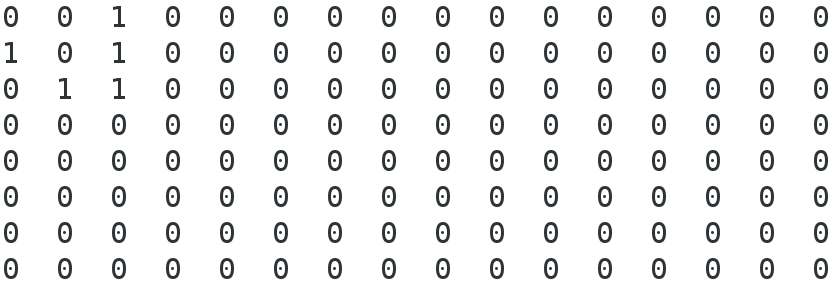
\includegraphics[width=7cm]{./images/OpenCAL/life_0000}
    \caption{Initial configuration of Game of Life, as implemented in Listing \ref{lst:cal_life}.}
    \label{fig:life_0000}
  \end{center}

    \begin{center}
    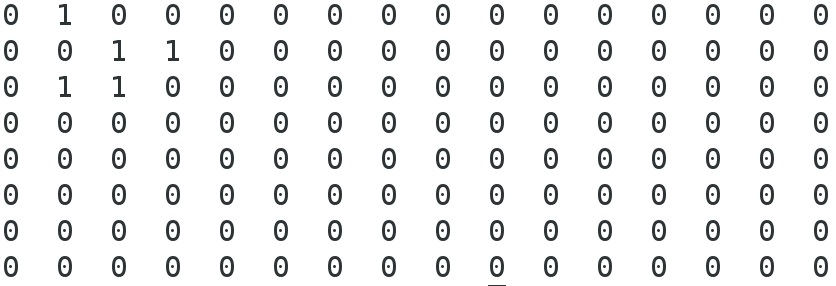
\includegraphics[width=7cm]{./images/OpenCAL/life_LAST}
    \caption{Final configuration of Game of Life (actually, just one step of computation), as implemented in Listing \ref{lst:cal_life}.}
    \label{fig:life_LAST}
  \end{center}
\end{figure}

%% \begin{figure}
%%   \begin{center}
%%     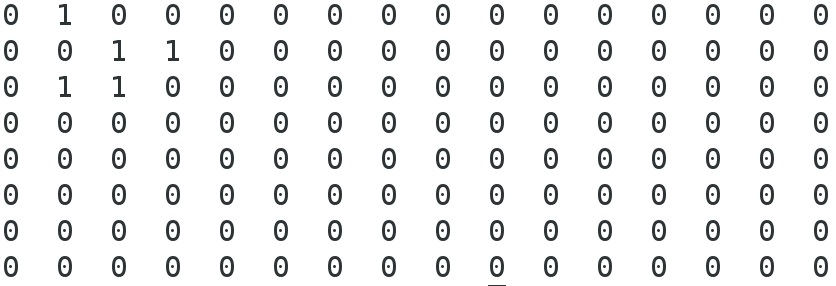
\includegraphics[width=7cm]{./images/OpenCAL/life_LAST}
%%     \caption{Final configuration of Game of Life (actually, just one step of computation), as implemented in Listing \ref{lst:cal_life}.}
%%     \label{fig:life_LAST}
%%   \end{center}
%% \end{figure}


\section{Custom Neighborhoods}\label{sec:CustomNeiughbourhoods}
In the Game of Life example, we used the predefined Moore
neighborhood. As already stated, OpenCAL also provides other 2D and 3D
predefined neighborhoods (cf. Listings \ref{lst:CALNeighborhood2D} and
\ref{lst:CALNeighborhood3D}). Furthermore, it allows for the
definition of custom neighborhood patterns.


%% \begin{lstlisting}[float, label=lst:calAddNeighbor2D-3D, caption=The calAddNeighbor2D() and calAddNeighbor3D() functions to define custom neighborhood patterns., numbers=none]
%%   struct CALCell2D*  calAddNeighbor2D(
%%       struct CALModel2D* ca2D,          // pointer to a 2D CA object
%%       int i,                            // row coordinate
%%       int j                             // column coordinate
%%   );

%%   struct CALCell3D*  calAddNeighbor3D(
%%       struct CALModel3D* ca3D,          // pointer to a 3D CA object
%%       int i,                            // row coordinate
%%       int j,                            // column coordinate
%%       int k                             // slice coordinate
%%   );
%% \end{lstlisting}


\begin{lstlisting}[float, label=lst:calAddNeighbor2D(), caption=The calAddNeighbor2D() functions to define custom neighborhood patterns in 2D CA., numbers=none]
  struct CALCell2D*  calAddNeighbor2D(
      struct CALModel2D* ca2D,          // pointer to a 2D CA object
      int i,                            // row coordinate
      int j                             // column coordinate
  );
\end{lstlisting}

\begin{lstlisting}[float, label=lst:calAddNeighbor3D(), caption=The calAddNeighbor3D() function to define custom neighborhood patterns in 3D CA., numbers=none]
  struct CALCell3D*  calAddNeighbor3D(
      struct CALModel3D* ca3D,          // pointer to a 3D CA object
      int i,                            // row coordinate
      int j,                            // column coordinate
      int k                             // slice coordinate
  );
\end{lstlisting}


In order to define a custom neighborhood pattern,
\verb'CAL_CUSTOM_NEIGHBORHOOD_2D' (or
\verb'CAL_CUSTOM_NEIGHBORHOOD_3D' in case of a 3D CA) must be used as
the third parameter of the \verb'calCADef2D()' function
(\verb'calCADef3D()' for a 3D CA). By doing this, you will start with an
empty neighboring pattern and can subsequently call the
\verb'calAddNeighbor2D()' (\verb'calAddNeighbor3D()' for 3D CA)
function to add a cell to the pattern (cf. Listings
\ref{lst:calAddNeighbor2D()} and \ref{lst:calAddNeighbor3D()}).

\begin{lstlisting}[float, label=lst:CustomMooreExample, caption=Example of custom neighbourhood pattern; the sequence of calls to the calAddNeighbor2D() function defines the Moore neighbourhood for the Game of Life CA., numbers=none]
  // ...
  int main ()
  {
    // define of the life CA and life_simulation simulation objects
    life = calCADef2D (8, 16, CAL_MOORE_NEIGHBORHOOD_2D, CAL_CUSTOM_NEIGHBORHOOD_2D , CAL_NO_OPT );
    //...

    //add neighbors of the Moore neighborhood
    calAddNeighbor2D(life,   0,   0); // neighbor 0 (central cell)
    calAddNeighbor2D(life, - 1,   0); // neighbor 1
    calAddNeighbor2D(life,   0, - 1); // neighbor 2
    calAddNeighbor2D(life,   0, + 1); // neighbor 3
    calAddNeighbor2D(life, + 1,   0); // neighbor 4
    calAddNeighbor2D(life, - 1, - 1); // neighbor 5
    calAddNeighbor2D(life, + 1, - 1); // neighbor 6
    calAddNeighbor2D(life, + 1, + 1); // neighbor 7
    calAddNeighbor2D(life, - 1, + 1); // neighbor 8

    //...
  }
\end{lstlisting}

Listing \ref{lst:CustomMooreExample} shows an example of how a custom
neighborhood pattern can be built for the Game of Life CA described
above. In particular, the Moore neighborhood is built by using a
sequence of nine calls to the \verb'calAddNeighbor2D()' function. The
first time the function is called, it adds the relative coordinates
(0,0) to the neighboring pattern. This first set of coordinates
receives the subscript identifier 0 and therefore can be used later to
refer the central cell. For instance, if
\verb'calSet2Di(life,Q,i,j,0)' is called, as at line 23 of Listing
\ref{lst:cal_life}, the relative coordinates of the neighbor 0
(specified as last parameters), i.e. (0,0), are added to the
coordinates of the cells the elementary process is applying to,
i.e. (i,j) (cf. second and third to last parameters), by obtaining the
cell (i,j) itself, which corresponds to the central cell by
definition. The subsequent calls to \verb'calAddNeighbor2D()' add
further couples of coordinates to the neighboring pattern, by
progressively assigning an integer subscript handle to each of
them.

Eventually, note that it is possible to define custom neighborhoods
starting from a predefined one. For instance, by considering the above
Game of Life example, it is possible to specify the value
\verb'CAL_MOORE_NEIGHBORHOOD_2D' as parameter for the
\verb'calCADef2D' function and then add further neighbors by calling
\verb'calAddNeighbor2D()' as many times the as the number of cells
have to be added.

\section{SciddicaT}\label{sec:sciddicaT}
In the previous section we illustrated an OpenCAL implementation of a
simple cellular automaton, namely the Conway’s Game of Life. Here, we
will deal with a more complex example concerning the implementations
of the Sciddica.

Sciddica is a family of two-dimensional XCA (cf. Chapter \ref{ch:CA})
debris flow models, successfully applied to the simulation of many
real cases, such as the 1988 Mt. Ontake (Japan) landslide and the 1998
Sarno (Italy) disaster. A simplified toy-version of Sciddica
(SciddicaT in the following) was here considered to be implemented in
\verb"OpenCAL", and its application to the 1992 Tessina (Italy)
landslide shown. Different versions will be presented, ranging from a
naive to a fully optimized implementation.

\subsection{SciddicaT naive implementation}

The first, naive, version of SciddicaT here considered is formally
defined as:

$$SciddicaT_{naive} = < R, X, Q , P, \sigma  >$$

where:

\begin{itemize}

\item $R$ is the set of points, with integer coordinates, which
  defines the 2-dimensional cellular space over which the phenomenon
  evolves. The generic cell in $R$ is individuated by means of a
  couple of integer coordinates $(i, j)$, where $0 \leq i < i_{max}$
  and $0 \leq j < j_{max}$. The first coordinate, $i$, represents the
  row, while the second, $j$, the column. The cell at coordinates
  $(0,0)$ is located at the top-left corner of the computational grid.

\item $X = \{(0,0), (-1, 0), (0, -1), (0, 1), (1, 0)\}$ is the von
  Neumann neighborhood relation (cf. Figure \ref{fig:2Dneighborhood}), a
  geometrical pattern which identifies the cells influencing the state
  transition of the central cell. The neighborhood of the generic cell
  of coordinate $(i, j)$ is given by
$$N(X, (i, j)) =$$
$$= \{(i, j)+(0,0), (i, j)+(-1, 0), (i, j)+(0, -1),
(i, j)+(0, 1), (i, j)+(1, 0)\} =$$
$$= \{(i, j), (i-1, j), (i, j-1), (i, j+1), (i+1, j)\}$$

Here, a subscript operator can be used to index cells belonging to the
neighborhood. Let $|X|$ be the number of elements in X, and $n \in
\mathbb{N}$, $0 \leq n < |X|$; the notation

$$N(X, (i, j), n)$$

represents the $n^{th}$ neighborhood of the cell $(i,j)$. Thereby, $N(X, (i, j), 0) = (i, j)$, i.e. the central cell, $N(X, (i, j), 1) = (i-1, j)$, i.e. the first neighbor, and so on.

\item $Q$ is the set of cell states. It is subdivided in the following
  substates:

\begin{itemize}
    \item   $Q_z$ is the set of values representing the topographic altitude (i.e. elevation);
    \item   $Q_h$ is the set of values representing the debris thickness;
    \item   $Q_o^4$ are the sets of values representing the debris outflows from the central cell to the neighboring ones.
\end{itemize}

The Cartesian product of the substates defines the overall set of
states $Q$:

$$Q = Q_z \times Q_h \times Q_o^4$$
so that the cell state is specified by the following sextuplet:

$$ q = (q_z, q_h, q_{o_0}, q_{o_1}, q_{o_2}, q_{o_3})$$
In particular, $q_{o_0}$ represents the outflows from the central cell towards the neighbor 1, $q_{o_1}$ the outflow towards the neighbor 2, and so on.

\item   $P$ is set of parameters ruling the CA dynamics:

\begin{itemize}
    \item   $p_\epsilon$ is the parameter which specifies the thickness of the debris that cannot leave the cell due to the effect of adherence;
    \item   $p_r$ is the relaxation rate parameter, which affects the size of outflows (cf. section above).
\end{itemize}

\item $\sigma : Q^5 \shortrightarrow Q$ is the deterministic cell
  transition function. It is composed by two elementary processes,
  listed below in the same order they are applied:
\begin{itemize}
\item $\sigma_1 : (Q_z \times Q_h)^5 \times p_\epsilon \times
  p_r\shortrightarrow Q_o^4$ determines the outflows from the central
  cell to the neighboring ones by applying the \emph{minimization
    algorithm of the differences}. In brief, a preliminary control
  avoids outflows computation for those cells in which the amount of
  debris is smaller or equal to $p_\epsilon$, acting as a
  simplification of the adherence effect. Thus, by means of the
  minimization algorithm, outflows $q_o(0,m) \; (m=0,\ldots,3)$ from
  the central cell towards its four adjacent cells are evaluated, and
  the $Q_o^4$ substates accordingly updated. Note that, $q_o(0,0)$
  represents the outflow from the central cell towards the neighbor
  1, $q_o(0,1)$ the outflow towards the neighbor 2, and so on. In
  general, $q_o(0,m)$ represents the outflows from the central cell
  towards the $n=(m+1)^{th}$ neighboring cell. Eventually, a
  relaxation rate factor, $p_r \in \; ]0,1]$, is considered in order
      to obtain the local equilibrium condition in more than one CA
      step. This can significantly improve the realism of model as, in
      general, more than one step may be needed to displace the proper
      amount of debris from a cell towards the adjacent ones. In this
      case, if $f(0,m) \; (i=0, \ldots, 3)$ represent the outgoing
      flows towards the 4 adjacent cells, as computed by the
      minimization algorithm, the resulting outflows are given by
      $q_o(0,m)=f(0,m) \cdot p_r \; (i=0, \ldots, 3)$.

      %% , while the amount of debris remaining in the central cell is
      %% obtained as: $$h_r(0) = q_0(0,0) = h(0) - \sum_{i=1}^4
      %% q_4(0,i)$$

\item $\sigma_2: Q_h \times (Q_o^4)^4 \shortrightarrow Q_h$ determines
  the value of debris thickness inside the cell by considering mass
  exchange in the cell neighborhood: $h'(0) = h(0) + \sum_{m=0}^3
  (q_o(0,m) - q_o(m,0))$. Here, $h'(0)$ is the new debris
  thickness inside the cell, while $q_o(m,0)$ represents the inflow from
  the $n=(m+1)^{th}$ neighboring cell. No parameters are involved in
  this elementary process.

\end{itemize}
\end{itemize}

In the following Listing \ref{lst:cal_sciddicaT}, an OpenCAL
implementation of SciddicaT is shown.

\lstinputlisting[label=lst:cal_sciddicaT, caption=An OpenCAL implementation of the SciddicaT debris flows simulation model.]{../opencal-examples/OpenCAL/cal_sciddicaT/source/sciddicaT.c}

As for the case of Game of Life, the CA model and the simulation
objects are declared as global variables (lines 22 and 35,
respectively), and defined later into the main function (lines 147 and
148, respectively). As can be seen, the 2D cellular space is a grid
of \verb'ROWS' rows times \verb'COLS' columns cells, corresponding to
$i_{max}$ and $j_{max}$ of the formal definition, respectively
(cf. lines 10-11), and the von Neumann neighborhood is adopted. The
cellular space is still toroidal, as in $Life$, and no optimization is
considered. Regarding the simulation object, a total of \verb'STEPS'
steps (i.e. 4000 steps - cf. line 14) are set, and implicit substates
updating considered.

Substates and parameters are grouped into two different C structures
(lines 24-28 and 30-33, respectively). Substates are therefore bound to
the CA context by means of the \verb'calAddSubstate2Dr()' function
(lines 155-160), as well as elementary processes are defined as
callback functions by means of the \verb'calAddElementaryProcess2D()'
function (lines 151-152).

The topographic altitude and debris thickness substates are
initialized from files through the \verb'calLoadSubstate2Dr()'
function (lines 163-164), while the remaining initial state of the CA
is set by means of the \verb'calRunAddInitFunc2D()' function. It
registers the \verb'sciddicaTSimulationInit()' callback, which is
executed once before the execution of the simulation loop, in which
the elementary processes are applied to the whole set of cells of the
cellular space. Such callback function must return void and take a
pointer to a simulation object as parameter. Differently to an
elementary process, which can only access state values of cells
belonging to the neighborhood, this function can perform global
operations over the whole cellular space. In the specific case of the
$SciddicaT_{naive}$ model, the \verb'sciddicaTSimulationInit()'
function (lines 104-130) sets the values of all the outflows from the
central cell to its neighbors to zero, by means of the function
\verb'calInitSubstate2Dr()' (lines 110-113). Moreover, it sets the
values of the P.r and P.epsilon parameters (lines 116-117) and
initializes the debris flow source by simply subtracting the source's
debris thickness to the topographic altitude. For this purpose, a
nested double \verb'for' is executed to check the debris thickness in
each cell of the cellular space. Here, the \verb'sciddicaT->rows' and
\verb'sciddicaT->cols' members of the CA object are used, which
represent the cellular space values of rows and columns,
respectively. Still, the \verb'calGet2Dr()' and \verb'calSet2Dr()'
functions are here employed to read/update substates' values inside
the cells.

Line 168 registers a \emph{steering} callback by means of the
\verb'calRunAddSteeringFunc2D()' function. Steering is executed at the
end of each computational step (i.e. after all the elementary
processes have been applied to each cell of the cellular space), and
can perform global operations over the whole cellular space. The
steering callback prototype must return void and take a pointer to a
simulation onject, as for the \verb'sciddicaTSteering()' callback
(lines 132-140). In the specific case of $SciddicaT_{naive}$, the
steering callback simply sets to zero outflows everywhere through the
\verb'calInitSubstate2Dr()' function.

The function \verb'calRun2D()' (line 171) enters the OpenCAL
simulation loop, which executes a total of 4000 steps (cf. lines 14
and 148). Eventually, the final debris flow path is saved to file by
means of the \verb'calSaveSubstate2Dr()' function (line 176) and
previously allocated memory is released (lines 179-180).

As regards the elementary processes, the first one, $\sigma_1$, is
defined at lines 38-88, while the second, $\sigma_2$, at lines
91-101. In both cases, the \verb'calGet2Dr()' \verb'calGetX2Dr()'
functions are employed to get values for the central cell and its
neighbors, respectively. Moreover, the \verb'calSet2Dr()' function,
updates the central cell state.

Figure \ref{fig:sciddicaT} shows the $SciddicaT_{naive}$ simulation of the 1992
Tessina (Italy) landslide. Both the initial landslide source and the
final flow path configuration are shown.

\begin{figure}[htbp]
  \centering
  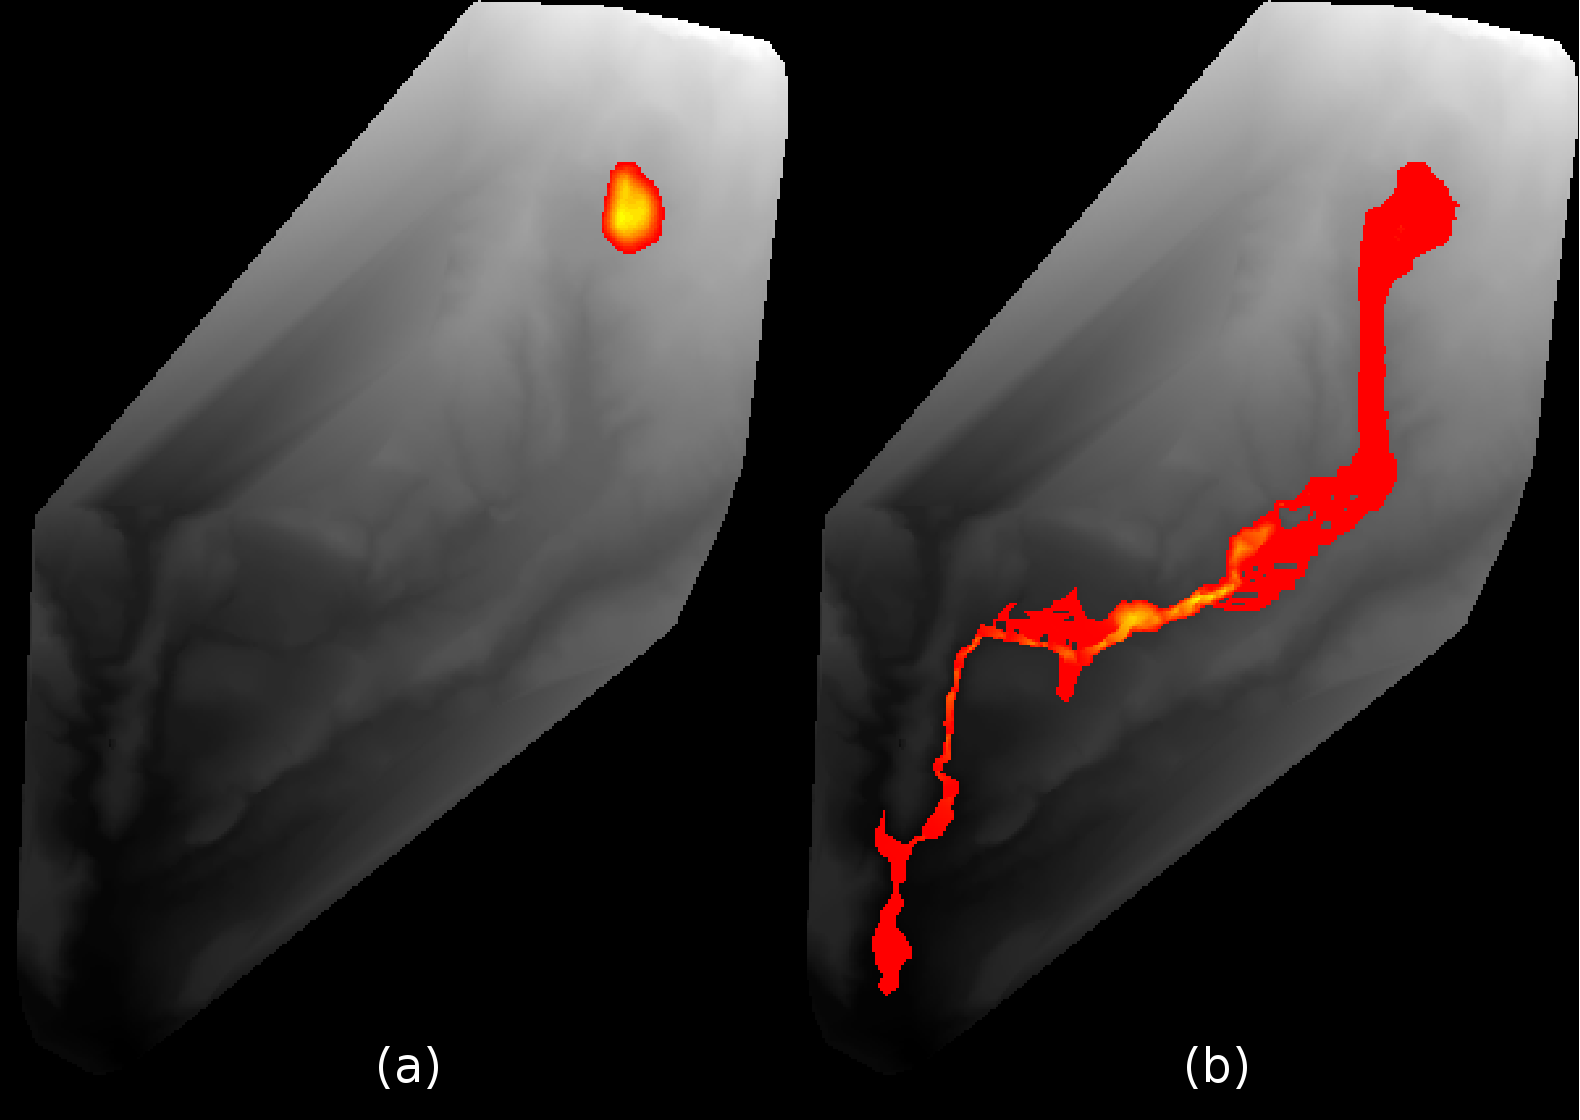
\includegraphics[width=11.5cm]{./images/OpenCAL/sciddicaT}
  \caption{$SciddicaT_{naive}$ simulation of the 1992 Tessina (Italy)
    landslide. Topographic altitudes are represented in gray
    scale. Black represents the lower altitude, while the white color
    is used for the highest elevation in the study area. Debris
    thickness is represented with colors ranging from red (for lower
    values) to yellow (for higher values). (a) Initial
    configuration. (b) Final debris flow path. Note that the graphic
    output was generated by using the \texttt{cal\_sciddicaT-glut}
    application, that implements the $SciddicaT_{naive}$ model and
    provides a minimal visualization system. You can find
    \texttt{cal\_sciddicaT-glut} in the examples directory.}
  \label{fig:sciddicaT}
\end{figure}

As regards computational performance, the simulation shown in Figure
\ref{fig:sciddicaT} was executed on an Intel Core i7-4702HQ CPU @
2.20GHz by exploiting only a single core. The simulation lasted a
total of 172 seconds and considered a total of 4000 computational
steps.


\subsection{SciddicaT with active cells optimization}\label{sec:sciddicaT_active}
In this section we present a computationally improved version of
SciddicaT, which takes advantage of the built-in OpenCAL active cells
optimization. As stated above, this optimization is able to restrict
computation to a subset of cells which are actually involved in
computation, by neglecting those cells that will not change state to
the next step (stationary cells).

In the case of SciddicaT, only cells containing debris and their
neighbors can change state to the next step, as they can be
interested in mass variation due to outflows and inflows. At the
beginning of the simulation, we can simply initialize the set of
active cells to those cells containing debris (i.e. those cells
forming the initial landslide source). Moreover, we can add to this
set new cells or remove some ones from it. Specifically, if an outflow
is computed from an active cell towards a neighboring non-active
cell, this latter can be added to the set of active cells and
considered for state change by the remaining elementary processes in
the current computation step \footnote{Remember that, by default,
  substates are updated after the application of each elementary
  process.} (if any), or by the next computational step. Similarly, if
a given active cell looses a sufficient amount of debris, it can be
eliminated from the set of active cells. In the case of SciddicaT,
this happens when its thickness becomes lower than or equal to a given
threshold (i.e. $p_\epsilon$).

In order to account for these processes, we have to slightly revise
the SciddicaT definition. In particular we have to add the set of
active cells, A. The optimized SciddicaT model is now defined as

$$SciddicaT_{ac} = < R, A, X, Q , P, \sigma >$$
where $A \subseteq R$ is the set of active cells, while the other
components are defined as before. The transition function is now defined as:

$$\sigma : A \times Q^5 \shortrightarrow Q \times A$$ denoting that it
is applied to only the cells in $A$ and that it can add/remove active
cells. More in detail, the $\sigma_1$ elementary process has to be
modified, as it can activate new cells. Moreover, a new elementary
process, $\sigma_3$, has to be added in order to remove cells that
cannot produce outflows during the next computational step due to the
fact that their debris thickness is negligible. The new sequence of
elementary processes is listed below, in the same order they are
applied.

\begin{itemize}
\item $\sigma_1 : A \times (Q_z \times Q_h)^5 \times p_\epsilon \times p_r
  \shortrightarrow Q_o^4 \times A$ determines the outflows from the
  central cell to the neighboring ones, as before. In addition, each
  time an outflow is computed, the neighbor receiving the flow is
  added to the set of active cells.

\item $\sigma_2: A \times Q_h \times (Q_o^4)^4 \shortrightarrow Q_h$ determines
  the value of debris thickness inside the cell by considering mass
  exchange in the cell neighborhood. This elementary process does not
  change with respect to the $SciddicaT_{naive}$ version.

\item $\sigma_3: A \times Q_h \times p_\epsilon \shortrightarrow A$
  removes a cell from $A$ if its debris thickness is lower than or
  equal to the $p_\epsilon$ threshold.
\end{itemize}

In order to implement the $SciddicaT_{ac}$ debris flows model in
OpenCAL, we have to change the definition of the CA object, by also
adding the third $\sigma_3$ elementary process. Moreover, the
$\sigma_1$ elementary process has to be changed. A complete
implementation of the active cells optimized version of SciddicaT is
shown in Listing \ref{lst:cal_Sciddicat-activecells} for the sake of
completeness, even if only the differences with respect to the
original implementation are commented.


\lstinputlisting[label=lst:cal_Sciddicat-activecells, caption=An OpenCAL implementation of the $SciddicaT_{ac}$ debris flows simulation model with the active cells optimization.]{../opencal-examples/OpenCAL/cal_sciddicaT-activecells/source/sciddicaT.c}


As noted, few modifications to the original source code are needed to
add the active cells optimization. In particular, the active cells
support is enabled by means of the \verb'CAL_OPT_ACTIVE_CELLS'
parameter at line 159, while the third elementary process added at
line 165. As regards the elementary process $\sigma_1$, it is the same
of that adopted in $SciddicaT_{naive}$, with the exception that when
an outflow is generated, the cell receiving the flow is added to the
set A of the active cells (line 88). Accordingly, note that the
\verb'calAddActiveCellX2D()' function at line 87 can be considered as
an unsafe, as it affects the activation state of a neighbor. Moreover,
an active cell is eliminated by the set A by means of the $\sigma_3$
elementary process in the case its debris thickness becomes lower than
or equal to the $p_\epsilon$ threshold parameter (lines 107-108).

Regarding the computational performance, the same simulation shown in
Figure \ref{fig:sciddicaT} was executed using the $SciddicaT_{ac}$
implementation. Still, only a single core of the Intel Core i7-4702HQ
CPU was used, as before. The simulation lasted a total of 22 seconds,
versus 172 seconds obtained for the naive version, which is about 8
times faster. Indeed, this can be considered a very good result and
can easily obtained when the simulation involves only a limited subset
of the computational domain.

\subsection{SciddicaT with direct neighbors update}\label{sec:sciddicaT_extended}
OpenCAL allows for a further optimization by means of the so called
\emph{unsafe operations}, i.e. operations that are not strictly
permitted by the formal definition of Cellular Automata. Obviously, in
order to be well defined, a CA exploiting unsafe operations must be
equivalent to a CA that does not use them.

In the case of SciddicaT, we will permit the transition function to
update the state of the neighboring cells, while the CA formally only
allows for state change for the central one. When an outflow is
computed from the central cell towards a neighbor, the flow can be
immediately subtracted from the central cell and added to the
neighbor. This does not change the state of the system at the current
step, which is defined by the \emph{current} computational plane,
since updated values are written to the \emph{next} plane. As a
result, the \emph{current} plane is not corrupted by the unsafe
operation, and the \emph{next} plane is used for progressively
accounting mass variation inside the cells. By introducing such
feature, outflows do not need to be saved (e.g. into additional
substates) anymore, as they are used to account mass exchange directly
during outflows computation. As figured out, this can give rise to a
further performance improvement for the application. The
$SciddicaT_{ac+dnu}$ CA exploiting both the active cells optimization
and unsafe operations is formally defined as:


$$SciddicaT_{ac+dnu} = < R, A, X, Q , P, \sigma  >$$

where:

\begin{itemize}

\item $R$ is the set of points, with integer coordinates, which
  defines the 2-dimensional cellular space over which the phenomenon
  evolves. The generic cell in $R$ is individuated by means of a
  couple of integer coordinates $(i, j)$, where $0 \leq i < i_{max}$
  and $0 \leq j < j_{max}$. The first coordinate, $i$, represents the
  row, while the second, $j$, the column. The cell at coordinates
  $(0,0)$ is located at the top-left corner of the computational grid.

\item $A \subseteq R$ is the set of active cells, i.e. those cells
  actually involved in computation.

\item $X = \{(0,0), (-1, 0), (0, -1), (0, 1), (1, 0)\}$ is the von
  Neumann neighborhood relation (cf. Figure \ref{fig:2Dneighborhood}),
  a geometrical pattern which identifies the cells influencing the
  state transition of the central cell. The neighborhood of the
  generic cell of coordinate $(i, j)$ is given by
$$N(X, (i, j)) =$$
$$= \{(i, j)+(0,0), (i, j)+(-1, 0), (i, j)+(0, -1),
(i, j)+(0, 1), (i, j)+(1, 0)\} =$$
$$= \{(i, j), (i-1, j), (i, j-1), (i, j+1), (i+1, j)\}$$

Here, a subscript operator can be used to index cells belonging to the
neighborhood. Let $|X|$ be the number of elements in X, and $n \in
\mathbb{N}$, $0 \leq n < |X|$; the notation

$$N(X, (i, j), n)$$

represents the $n^{th}$ neighborhood of the cell $(i,j)$. Thereby,
$N(X, (i, j), 0) = (i, j)$, i.e. the central cell, $N(X, (i, j), 1) =
(i-1, j)$, i.e. the first neighbor, and so on (cf. Figure
\ref{fig:LifeNeighborhood}).

\item $Q$ is the set of cell states; it is subdivided in the following
  substates:

\begin{itemize}
    \item   $Q_z$ is the set of values representing the topographic altitude (i.e. elevation);
    \item   $Q_h$ is the set of values representing the debris thickness;
\end{itemize}

The Cartesian product of the substates defines the overall set of
state $Q$:

$$Q = Q_z \times Q_h$$
so that the cell state is specified by:

$$ q = (q_z, q_h)$$

\item   $P$ is set of parameters ruling the CA dynamics:

\begin{itemize}
    \item   $p_\epsilon$ is the parameter which specifies the thickness of the debris that cannot leave the cell due to the effect of adherence;
    \item   $p_r$ is the relaxation rate parameter, which affects the size of outflows (cf. section above).
\end{itemize}

\item $\sigma : A \times Q^5 \shortrightarrow Q$ is the deterministic cell
  transition function. It is composed by two elementary processes:
\begin{itemize}
\item $\sigma_1 : A \times (Q_z \times Q_h)^5 \times p_\epsilon \times
  p_r\shortrightarrow (A \times Q_h)^5$ determines the outflows from
  the central cell to the neighboring ones and updates debris
  thickness inside the central cell and its neighbors accordingly. It
  also adds the neighboring cells receiving a flow to the set A of the
  active cells.

\item $\sigma_2: A \times Q_h \times p_\epsilon \shortrightarrow A$ removes the
  cell from the set A of the active cells if the debris thickness
  inside the cell is lower than or equal to the $p_\epsilon$
  threshold.

\end{itemize}
\end{itemize}

Note that, only the topographic altitude and the debris thickness are
now considered as model substates, as the four outflows substates are
no longer needed. Moreover, the number of elementary process now
considered is two, instead of three for the previous versions of
SciddicaT. The OpenCAL implementation of $SciddicaT_{ac+dnu}$ is shown
in Listing \ref{lst:cal_sciddicaT-unsafe}.

\lstinputlisting[label=lst:cal_sciddicaT-unsafe, caption=An OpenCAL implementation of the SciddicaT debris flows simulation model with both the active cells optimization and the direct neighbors upddate unsafe operation.]{../opencal-examples/OpenCAL/cal_sciddicaT-unsafe/source/sciddicaT.c}

As noted, the definitions of CA and simulation objects doesn't
change from the previous implementation (lines 131-132), while only
two elementary processes are considered (lines 135-136). In
particular, the first call to \verb'calAddElementaryProcess2D()'
registers the callback function implementing the $\sigma_1$ elementary
process. It computes outflows from the (active) central cell to its
neighbors (line 83) and updates the debris thickness in both the
central cell and the neighboring cell receiving a flow (lines
84-85). Moreover, neighboring cells receiving a flow are added to the
set A of active cells (line 88) and therefore will be considered for
elaboration by the subsequent elementary process ($\sigma_2$) in the
current step of computation\footnote{This is due to the fact that a
  substates' update is performed after the first elementary process
  has been applied to all the (active) cells of the cellular
  space. This behavior is set by means of the
  \texttt{CAL\_UPDATE\_IMPLICIT} parameter used in the definition of
  the simulation object at line 132 of Listing
  \ref{lst:cal_sciddicaT-unsafe}.}. In particular, the
\verb'calSetX2Dr()' \emph{unsafe} function is used to update the
debris thickness of the neighboring cells receiving a flow, while the
\verb'calAddActiveCellX2D()' function is used to add a neighboring
cells receiving a flow to the set $A$ of active cells.  The $\sigma_2$
elementary process, simply removes inactive cells from $A$ (lines
95-86), as in the previous example.


Substates are added to the CA at lines 139-140. Here, the first
substate, $Q_z$, is added by means of the
\verb'calAddSingleLayerSubstate2Dr()' function, here considered
to allocate memory only for the \emph{current} computing plane. In
fact, topographic altitude only changes at the simulation
initialization stage (cf. lines 147 and 117), while it remains
unchanged during computation as its value is never updated by the
transition function. This allows for memory space allocation
optimization and possibly for computational performance
improvements. Note that, at line 117 we used the
\verb'calSetCurrent2Dr()' function, instead of the usual
\verb'calSet2Dr()'. The \verb'calSetCurrent2Dr()' function allows for
updating the \emph{current} computational plane (the only present in
the $Q_z$ substate), while \verb'calSet2Dr()' would update the
\emph{next} computational plane, by producing an access violation
error.

Regarding the computational performance, the same simulation shown in
Figure \ref{fig:sciddicaT} was executed by considering
$SciddicaT_{ac+dnu}$ on a single core of the same Intel core i7
processor. The simulation lasted a total of 11 seconds, versus 22
seconds obtained for SciddicaT_{ac} and 172 seconds for
SciddicaT_{naive}, with speed up of 2 and 16, respectively.



\subsection{SciddicaT with explicit simulation loop}
Even if results obtained so far can be considered more than
satisfying, it is further possible to improve computational
performance of SciddicaT by avoiding unnecessary substates
updating. In fact, in some cases, elementary processes do not affect
one or more model substates and therefore their updating can be
avoided.

As we stated above, when we use the implicit \verb'calRun2D()'
simulation loop, an update of all the defined substates is executed at
the end of each elementary process. However, this behavior can be
modified by making the OpenCAL simulation loop explicit.

In the specific case of the above implementation of SciddicaT, the
second elementary process, $\sigma_2$, just removes cells that became
inactive from the set $A$ of active cells and doesn't affect the
mode's substates\footnote{Actually, only $Q.h$ can be update by the
  transition function, since $Q.z$ is a single-layered substate.}. As
a consequence, no substates updating is needed after the application
of $\sigma_2$. Being substates updating a time consuming operation,
this can further speed up your simulation.

The new $SciddicaT_{ac+dnu+esl}$ OpenCAL implementation of SciddicaT,
which take adavantage of an explicit simulation loop, avoiding
unnecessary substate updating, is presented in Listing
\ref{lst:cal_sciddicaT-explicit}. It also shows how a generic stopping
criterion can be defined.


\lstinputlisting[label=lst:cal_sciddicaT-explicit, caption=An OpenCAL implementation of the $SciddicaT_{ac+dnu+esl}$ debris flows simulation model with the active cells optimization, the direct neighbors update, and an explicit simulation loop.]{../opencal-examples/OpenCAL/cal_sciddicaT-unsafe-explicit/source/sciddicaT.c}


As noted, the \verb'calRunAddGlobalTransitionFunc2D()' function is
called to register a custom transition function callback (line
177). In the specific case of SciddicaT, the
\verb'sciddicaTransitionFunction()' callback (lines 132-143) is used
to make the elementary processes application and the substates update
explicit. Here, the elementary processes are applied in the same order
they are defined by means of the \verb'calAddElementaryProcess2D()'
function (which is the default behavior of OpenCAL), even if you are
free to re-order the call sequence within the explicit transition
function callback. In particular, the \verb'sciddicaTFlowsComputation()'
elementary process is applied to each (active) cell into the
computational domain by means of the
\verb'calApplyElementaryProcess2D()'. Then, the set $A$ of the active
cells and the $Q_h$ substate are updated by
\verb'calUpdateActiveCells2D()' and \verb'calUpdateSubstate2Dr()',
respectively\footnote{Note that active cells are updated first
  otherwise the subsequent substate update could neglect some cells
  that have become active during the current step. For instance,
  inactive cells can receive a flow and become active at the current
  step of computation. If the set of active cells is not updated
  before any other substates, those new cells will still be considered
  inactive during the current step and their value will not be
  updated, by losing debris flow mass.}. Eventually, the
\verb'sciddicaTRemoveInactiveCells()' elementary process is
applied, which only removes cells that became inactive during the
current computational step, and the set $A$ is accordingly updated.


As regards the computational performance, execution time of this
further optimized version lasted 12 seconds to complete the 4000 steps
required by the simulation on a single core of the same Intel Core i7
processor used before. The obtained speedup can seem quite small (less
than the 10\%) with respect to the previous implementation of
SciddicaT. However, it must be noted that SciddicaT is a very
simplified model and higher speedups can certainly be obtained for
more complex CA made up by more elementary processes, these latter
involving here only a small set of model substates, or by considering
larger CA spaces. Table \ref{tab:speedup} resumes computational
performance of all the above illustrated SciddicaT implementations.

\begin{table}
  \centering
  \begin{tabular}{l|c|c}
    \hline
    CA model & Elapsed time [s] & Speedup \\
    \hline
    $SciddicaT_{naive}$      & 240 & 1\\
    $SciddicaT_{ac}$         & 23  & 10.43\\
    $SciddicaT_{ac+dnu}$     & 13  & 18.46\\
    $SciddicaT_{ac+dnu+esl}$  & 12  & 20\\
    \hline
  \end{tabular}
  \caption{Computational performance of four different
    implementations of the SciddicaT debris flows model.}
  \label{tab:speedup}
\end{table}


\section{A three-dimensional example}\label{sec:mod2}

In order to introduce three-dimensional CA development with OpenCAL,
this section describes the implementation of a simple 3D model, namely
the \emph{mod2} 3D CA. In this model, cells can be in one of two
different states, 0 or 1, as in Game of Life. The cellular space is a
parallelepiped made by cubic cells, while the cell's neighborhood is
the 3D Moore one, consisting of the central cell and its adjacent
cells. The transition function simply evaluates the quantity $s$ as
the number of neighboring cells which are in the state 1 and sets the
new state for the central cell as $s\%2$ (i.e. the remainder of $s$
divided by 2). This simple example of 3D CA is formally defined as:

$$mod2 = < R, X, Q, \sigma >$$

where:

\begin{itemize}

\item $R$ is the set of points, with integer coordinates, which
  defines the 3-dimensional cellular space. The generic cell in $R$ is
  individuated by means of a triple of integer coordinates $(i, j,
  k)$, where $0 \leq i < i_{max}$, $0 \leq j < j_{max}$, and $0 \leq k
  < k_{max}$. The first coordinate, $i$, represents the row, the
  second, $j$, the column, while the third coordinate represents the
  slice. The cell at coordinates $(0,0,0)$ is located at the
  top-left-far corner of the computational grid.

\item $X = \{(0,0,0), \dots, (-1,1,0), (0,0,-1), \dots, (-1,1,-1),
  (0,0,1), \dots, (-1,1,1)\}$ is the Moore neighborhood
  relation, a geometrical pattern which identifies the cells
  influencing the state transition of the central cell. The
  neighborhood of the generic cell of coordinate $(i, j)$ is given by
  $$N(X, (i, j, k)) = $$
  $$= \{(i, j, k)+(0,0,0), \dots, (i, j, k)+(-1,1,-1)\} =$$
  $$= \{(i, j, k), \dots, (i-1,j+1,k-1)\}$$
  Here, a subscript operator can be used to index cells belonging to the
  neighborhood. Let $|X|$ be the number of elements in X, and $n \in
  \mathbb{N}$, $0 \leq n < |X|$; the notation

  $$N(X, (i, j, k), n)$$

  represents the $n^{th}$ neighborhood of the cell $(i,j,k)$. Thereby,
  $N(X, (i, j, k), 0) = (i, j, k)$, i.e. the central cell, $N(X, (i, j, k), 1)
  = (i-1, j, k)$, i.e. the first neighbor, and so on.

\item $Q = \{0, 1\}$ is the set of cell states.

\item $\sigma : Q^{27} \shortrightarrow Q$ is the deterministic cell
  transition function. It is composed by one elementary process, which
  implements the previously described transition rules.
\end{itemize}


As imagined, the OpenCAL implementation of the \emph{mod2} 3D
CA is very simple as the Conway's game of Life. The complete
source code is shown in Listing \ref{lst:cal_mod2CA3D}.


\lstinputlisting[label=lst:cal_mod2CA3D, caption=An OpenCAL implementation of the \emph{mod2} 3D CA.]{../opencal-examples/OpenCAL/cal_mod2CA3D/source/mod2CA3D.c}


Even if Listing \ref{lst:cal_mod2CA3D} is concise, it completely
defines the \emph{mod2} 3D CA and performs a simulation (actually,
only one step in this example). Lines 3-5 include some header files
for the 3D version of OpenCAL, while lines 12-14 declare CA, substate
and simulation objects. These are therefore defined later in the main
function. In particular, line 30 defines the CA as a parallelepiped
having \verb'ROWS' rows, \verb'COLS' columns and \verb'SLICES' slices
(cf. lines 7-9). Moreover, the 3D Moore neighborhood is here set as
well as cyclic conditions at boundaries. Eventually, no optimizations
are considered. The complete definition of \verb'calCADef3D()' is
provided in Listing \ref{lst:calCADef3D}. Line 31 defines the
simulation object by setting just one step of computation and implicit
substate update. The complete definition of \verb'calRunDef3D' is
provided in Listing \ref{lst:calRunDef3D()}. Finally, the only substate,
$Q$, is defined at line 34. Note that, since it was defined by means
of the \verb'calInitSubstate3Db()' function, each element $q \in Q$
results to be of the CALbyte type. Line 37 registers the one and only
CA elementary process, namely the \verb'mod2TransitionFunction()'
function, which is then implemented at lines 17-25. Line 43
initializes the cell's substate $Q$ at coordinates (2, 3, 1) to the
state 1. The obtained initial configuration is then saved at line 46,
and the simulation executed at line 49. The final configuration is
therefore saved at line 52 and, eventually, memory previously and
implicitly allocated is released at lines 55-56. Note that,
differently to the previous examples, almost all the OpenCAL functions
come in the 3D flower. For instance, this is the case of the
\verb'alGetX3Db()' and \verb'calSet3Db()' functions at lines 22 and
24, respectively, which take \verb'k' as third cell's coordinate,
identifying the cellular space's slice.

Figures \ref{fig:mod2_0000} and \ref{fig:mod2_LAST} show the initial
and final configuration of \emph{mod2} 3D CA as implemented in Listing
\ref{lst:cal_mod2CA3D}, respectively. A graphical representation after
77 computational step is shown in Figure \ref{fig:cal_mod2CA3D}.

\begin{figure}
  \begin{center}
    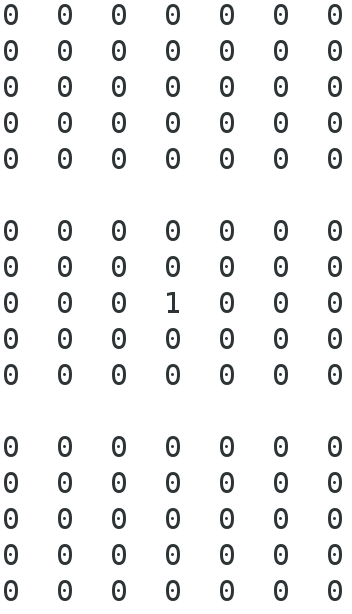
\includegraphics[width=3.5cm]{./images/OpenCAL/mod2_0000}
    \caption{Initial configuration of mod2 3D CA, as implemented in Listing \ref{lst:cal_mod2CA3D}.}
    \label{fig:mod2_0000}
  \end{center}
\end{figure}

\begin{figure}
  \begin{center}
    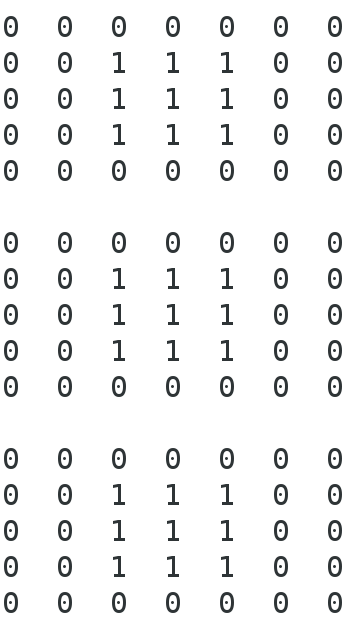
\includegraphics[width=3.5cm]{./images/OpenCAL/mod2_LAST}
    \caption{Final configuration of mod2 3D CA (actually, just one step of computation), as implemented in Listing \ref{lst:cal_mod2CA3D}.}
    \label{fig:mod2_LAST}
  \end{center}
\end{figure}


\begin{figure}
  \begin{center}
    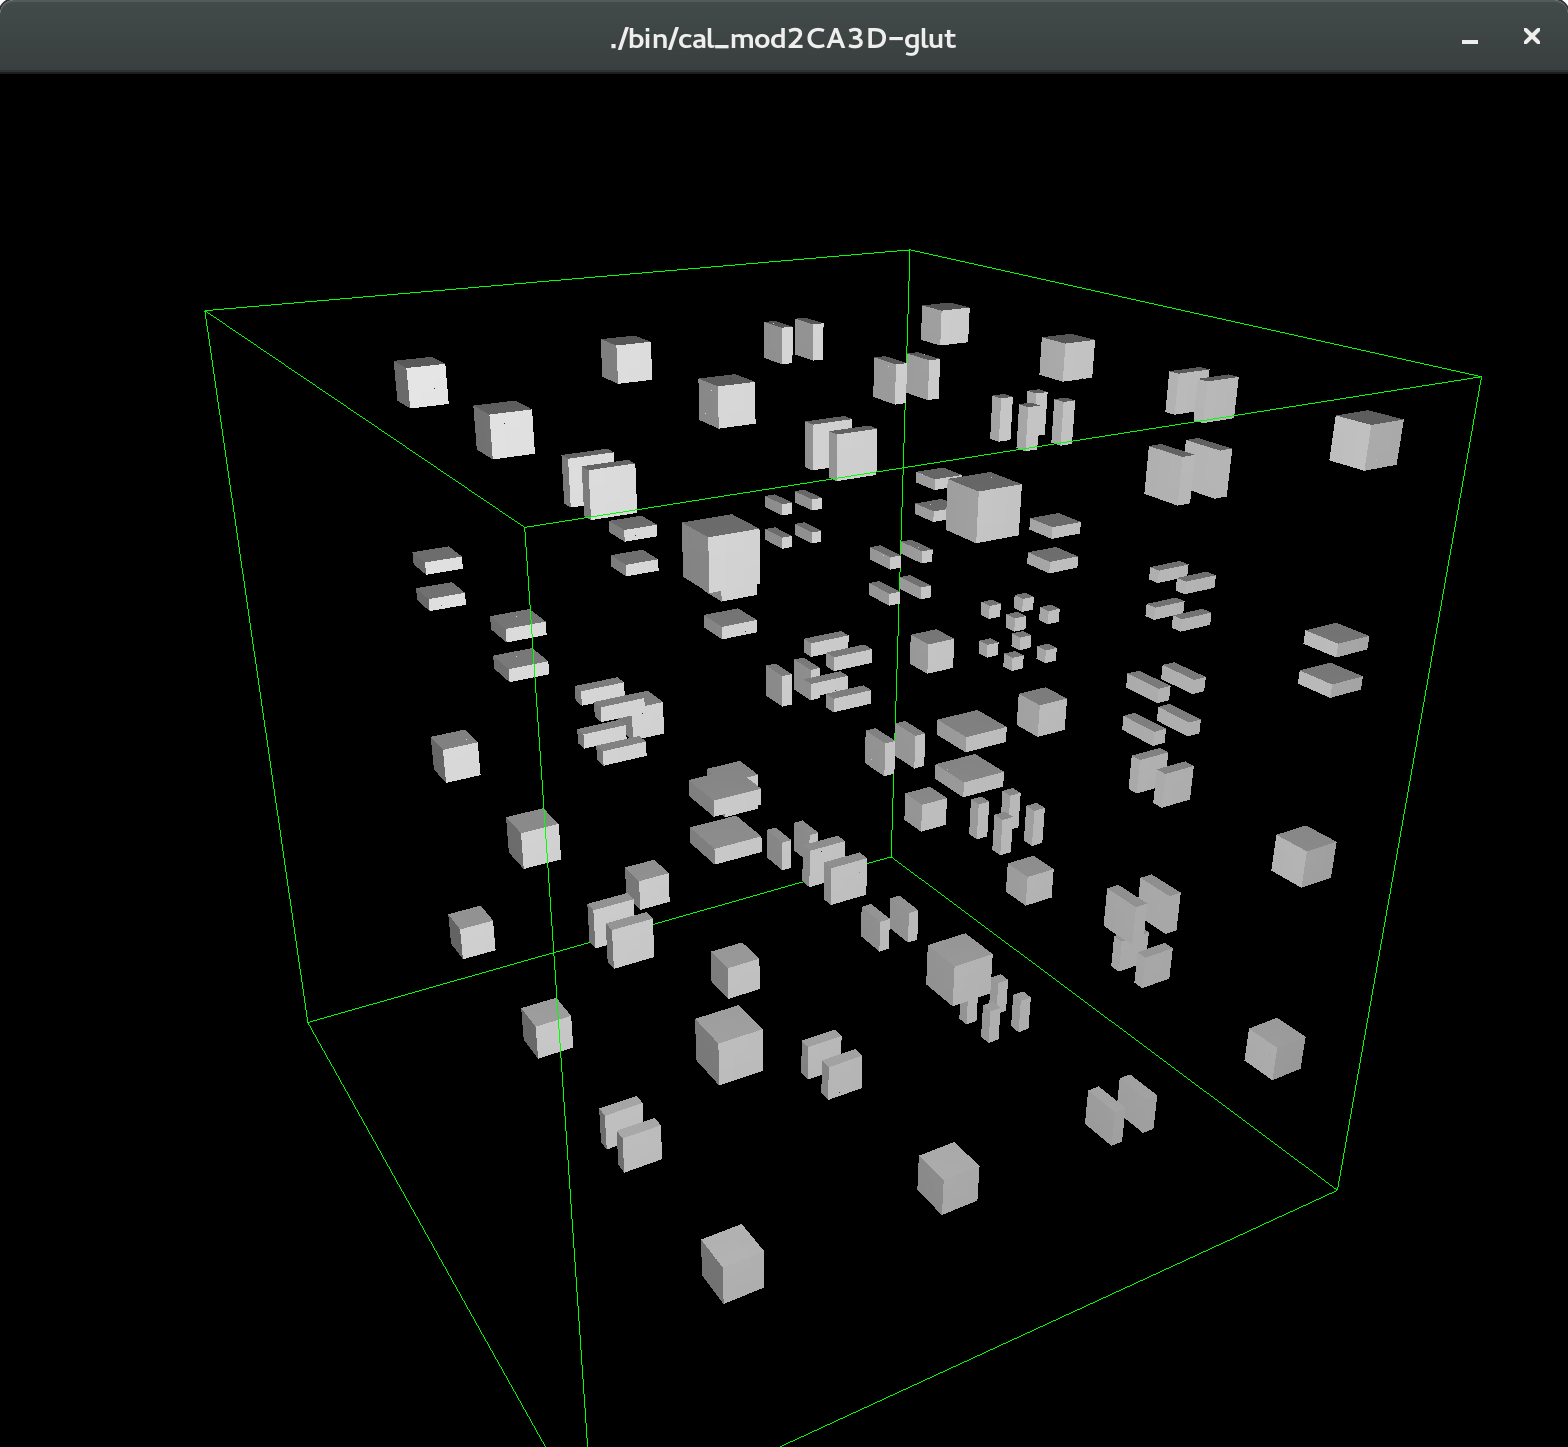
\includegraphics[width=12cm]{./images/OpenCAL/mod23DCA-glut}
    \caption{Graphical representation of the mod2 3D CA after 77 computational steps, as implemented in Listing \ref{lst:cal_mod2CA3D}. CA dimensions were set to (rows, cols, slices) = (65, 65, 65), while the initial seed located at coordinates (12, 12, 12). Cells in black are in the state 0, cell in white are in the state 1.}
    \label{fig:cal_mod2CA3D}
  \end{center}
\end{figure}


\section{Combining OpenCAL and OpenCAL-GL}\label{sec:combining_gl}

In this section, we will show how to combine the OpenCAL and
OpenCAL-GL libraries to obtain an immediate graphic output for your
simulation. For this purpose, here we re-propose two of the examples
presented above, namely the SciddicaT debris flow model and the
\emph{mod2} CA, by adding to them an OpenGL-based viewer in a
straightforward manner. Note that the graphic outputs for the
SciddicaT and \emph{mod2} CA shown above, were instead obtained by
means of non-integrated \emph{ad hoc} GLUT applications, which can be
found in the OpenCAL examples, together with others, ending with the
\verb'-glut' suffix.

\subsection{Implementing SciddicaT in OpenCAL and OpenCAL-GL}\label{sec:calgl_sciddicaT}

A new implementation of SciddicaT is presented in Listing
\ref{lst:calgl_sciddicaT}, which integrates a simple 2D and 3D
multi-view visualization system based on OpenCAL-GL. The complete
implementation is shown for the sake of completeness. A screenshot is
shown in Figure \ref{fig:calgl_sciddicaT1}.

\begin{figure}
  \begin{center}
    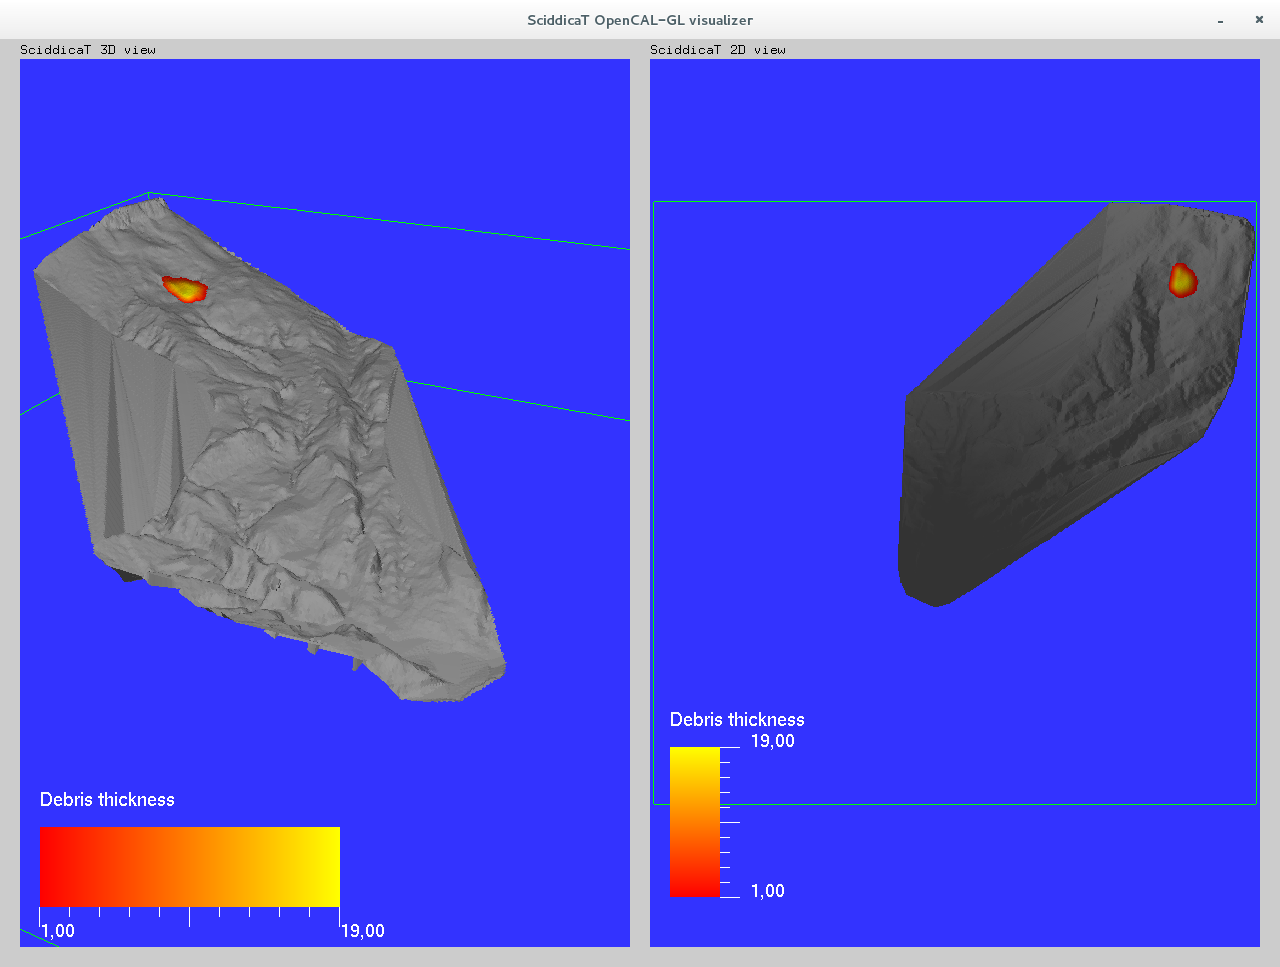
\includegraphics[width=12cm]{./images/OpenCAL/calgl_sciddicaT1}
    \caption{Screenshot of the SciddicaT debris flow model with a
      multi-view 2D and 3D visualization system based on OpenCAL-GL.}
    \label{fig:calgl_sciddicaT1}
  \end{center}
\end{figure}

\lstinputlisting[label=lst:calgl_sciddicaT, caption=An OpenCAL
  implementation of the sciddicaT CA with openCAL-GL graphic
  output.]{../opencal-examples/OpenCAL-GL/calgl_sciddicaT/source/sciddicaT.c}

As noticed, the \verb'OpenCAL-GL/calgl2D.h' and
\verb'OpenCAL-GL/calgl2DWindow.h' headers are included to use
OpenCAL-GL at lines 7-8, and two visualization objects (of type
\verb'CALDrawModel2D') are declared into the \verb'main()' function
at lines 170-171. Each of them allows to define a particular view for
the CA inside a graphic window.

The \verb'calglDefDrawModel2D()' function (lines 200, 218) is used to
initialize graphic objects. The first parameter specifies the type of
drawing to be considered and can assume the values listed in Table
\ref{tab:draw_modes}. If the \emph{basic} (or \emph{flat})
\emph{visualization model} is selected, substates are represented by
considering their actual dimensions. Accordingly, 2D substates are
represented as flat planes, as well as 3D substates as
parallelepipeds. At the contrary, if the \emph{surface model} is
selected, 2D substates will be represented in 3D by interpreting data
inside cells as altitude values (to be used along the $z$
coordinate). Note that the surface visualization model is valid for 2D
CA only. The second parameter is a label, representing the title of the
view within the graphic window. Eventually, the third parameter is a
pointer to the CA object to be visualized, while the last one is a
pointer to the corresponding simulation object.

\begin{table}
  \centering
  \footnotesize
  \begin{tabular}{l|l}
    \hline
    Drawing type & Meaning \\
    \hline
    \verb'CALGL_DRAW_MODE_FLAT'    & Basic substate representation \\
    \verb'CALGL_DRAW_MODE_SURFACE' & DEM-like representation \\
    \hline
  \end{tabular}
  \caption{Possible OpenCAL-GL drawing types. DEM is the acronym of Digital Elevation Model.}
  \label{tab:draw_modes}
\end{table}

To build a specific view, we can use the
\verb'calglAddToDrawModel2Dr()' function (lines 204-208). It adds a
node into a tree-based representation of the graphic view, where each
node has a link to a CA substate and specifies how this substate have
to be considered for representation. Specifically, the first parameter
is a pointer to a OpenCAL-GL visualization object, while the second
and third parameters are pointers to the parent node and the new node
to be created, respectively. The fourth parameter specifies how
substate data have to be interpreted, if as vertices (to be used to
geometrically represent the data), normal vectors\footnote{Normal
  vectors are obtained by scalar values representing vertices by means
  of cross product and normalization operations. They are only used
  for light calculation and are not displayed.} (to be used for light
calculation), or colors (to be used for shading purposes - cf. Table
\ref{tab:substate_type_info}). The fifth parameter specifies the color
scheme to be used. Possible values are listed in Table
\ref{tab:substate_color_info}. Eventually, the last parameter
specifies if the substate has to be considered static (i.e. it is not
updated during the simulation) or dynamic (i.e. values are modified by
the simulation). Please refer to Table
\ref{tab:substate_updating_type} for possible values. In general,
however, visualization of static substates is more efficient.

\begin{table}
  \centering
  \small
  \begin{tabular}{l|l}
    \hline
    Substate data interpretation & Meaning\\
    \hline
    \verb'CALGL_TYPE_INFO_VERTEX_DATA' & Vertex data\\
    \verb'CALGL_TYPE_INFO_NORMAL_DATA' & Normal data\\
    \verb'CALGL_TYPE_INFO_COLOR_DATA'  & Color data\\
    \hline
  \end{tabular}
  \caption{Possible OpenCAL-GL graphic interpretation for substate data.}
  \label{tab:substate_type_info}
\end{table}

\begin{table}
  \centering
  \footnotesize
  \begin{tabular}{l|l}
    \hline
    Substate color specification & Meaning \\
    \hline
    \verb'CALGL_TYPE_INFO_USE_CONST_VALUE' & Color is set by using the \verb'calglColor2D()' function\\
    \verb'CALGL_TYPE_INFO_USE_GRAY_SCALE'  & Gray gradient (white for the highest value)\\
    \verb'CALGL_TYPE_INFO_USE_RED_SCALE '  & Red gradient (red for the highest value)\\
    \verb'CALGL_TYPE_INFO_USE_GREEN_SCALE' & Green gradient (green for the highest value)\\
    \verb'CALGL_TYPE_INFO_USE_BLUE_SCALE'  & Blue gradient (blue for the highest value)\\
    \hline
  \end{tabular}
  \caption{Possible OpenCAL-GL substate color settings.}
  \label{tab:substate_color_info}
\end{table}

\begin{table}
  \centering
  \small
  \begin{tabular}{l|l}
    \hline
    Substate updating type & Meaning \\
    \hline
    \verb'CALGL_DATA_TYPE_DYNAMIC' & Dynamic data\\
    \verb'CALGL_DATA_TYPE_STATIC'  & Static data\\
    \hline
  \end{tabular}
  \caption{Possible substate data updating type.}
  \label{tab:substate_updating_type}
\end{table}

In the considered example (Listing \ref{lst:calgl_sciddicaT}), the
\verb'draw_model3D' object defines a 3D view for the CA, since the
first parameter of the \verb'calglDefDrawModel2D()' function is set to
\verb'CALGL_DRAW_MODE_SURFACE' (line 200) and, therefore, the substate
is interpreted as a 3D surface in which each cell contains an
altitude. The tree-based graphic representation is initialized at line
202, where the root node is defined and linked to the \verb'Q.z'
substate. It is assumed as the root node because its parent node is
set to \verb'NULL'. Moreover, the function specifies that the \verb'Q.z'
data has to be used as vertices, to be used to build a mesh
representation of the substate itself. Lines 204-205 attach two new
\emph{information nodes} to the parent, which corresponds to the root
node in this case, both of them having a link to the \verb'Q.z'
substate. In particular, line 204 sets the color to be used for
representing the root node (i.e. the topographic surface defined by
\verb'Q.z'). In this specific case, it is the one previously defined
at line 203. Instead, line 205 specifies that \verb'Q.z' have also to
be used for normal vectors calculation. Line 206 creates a further new
node and attaches it to the root again. In particular, this new node
links the \verb'Q.h' substate and sets its data to be used as
vertices. The hierarchy thus obtained makes that \verb'Q.h' is
represented above \verb'Q.z', such as two layers. Note that, in some
cases, due to approximations of the graphic rendering, layers can
intersect each other. In this cases, you can move up a layer by means of
the \verb'calglSetHeightOffset2D()' function, as done at line 205.

Lines 207-208 define
other information nodes for the \verb'Q.h' substate, specifically for
color and normal data. Figure \ref{fig:opencal_gl_tree_example} show
the tree obtained by considering the statements at lines 200-208 of
Listing \ref{lst:calgl_sciddicaT}.

\begin{figure}
  \begin{center}
    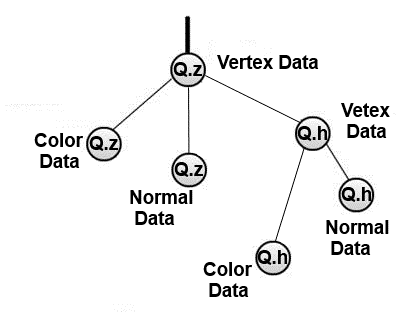
\includegraphics[width=5cm]{./images/OpenCAL/calgl_sciddicaT_tree_model}
    \caption{Tree-based representation of the 3D graphic view defined
      in Listing \ref{lst:calgl_sciddicaT} and shown in Figure
      \ref{fig:calgl_sciddicaT1}.}
    \label{fig:opencal_gl_tree_example}
  \end{center}
\end{figure}

The function \verb'calglInfoBar2Dr()' defines a legend for the
view. The first parameter is a pointer to the OpenCAL-GL view object,
while the second a pointer to a reference substate to associate the
resulting scalar-bar. The third parameter is a caption, while the
fourth specifies the color scheme to be used, that must be set
accordingly to the one used for the substate representation. The last
four parameters specify the position (in $x$ and $y$ coordinates with
respect to the lower-left corner of the graphic view within the
window) and extension for the legend (in pixels). In the considered
example, a legend for the \verb'Q.h' substate is defined and attached
to the \verb'draw_model3D' object at line 211.

Lines 218-220 of Listing \ref{lst:calgl_sciddicaT} define a further
view for the same CA. In particular, the first parameter of the
\verb'calglDefDrawModel2D()' function, which is set to
\verb'CALGL_DRAW_MODE_FLAT', specifies a 2D (i.e. flat)
representation, while the other view specifications are inherited from
the previously defined \verb'draw_model3D' object (line 219). A legend
is also defined at line 220.

Line 222 sets a vertical layout for arranging the two defined views
within the window, by means of the
\verb'calglSetLayoutOrientation2D()' function. Allowed layouts are
listed in Table \ref{tab:calgl_layouts}. If no layouts are specified,
OpenCAL-GL automatically arranges the defined views inside the graphic
window in a matrix layout.

\begin{table}
  \centering
  \small
  \begin{tabular}{l|l}
    \hline
    Possible values for view layouts & Meaning\\
    \hline
    \verb'CALGL_LAYOUT_ORIENTATION_HORIZONTAL' & Horizontal layout\\
    \verb'CALGL_LAYOUT_ORIENTATION_VERTICAL'   & Vertical layout\\
    \verb'CALGL_LAYOUT_ORIENTATION_UNKNOW'     & Automatic layout\\
    \hline
  \end{tabular}
  \caption{Possible OpenCAL-GL graphic interpretation for substate data.}
  \label{tab:calgl_layouts}
\end{table}

The \verb'calglMainLoop2D()' function (line 226) enters the
application main loop. It corresponds to the GLUT main loop and
executes both the simulation steps and the graphic rendering. As a
result, the application's execution flow never returns to the
\verb'main()' function and therefore, to manage memory deallocation
and other possible operations, a callback function is defined and
executed just before program termination, namely \verb'exitFunction()'
(lines 157-165). It was registered at line 173 through the
\verb'atexit()' function. Note that, if you do not want visualize all
the computational steps, you can call the \verb'calglSetDisplayStep()'
function to specify a refreshing interval in steps (cf. line 224).

\begin{figure}
  \begin{center}
    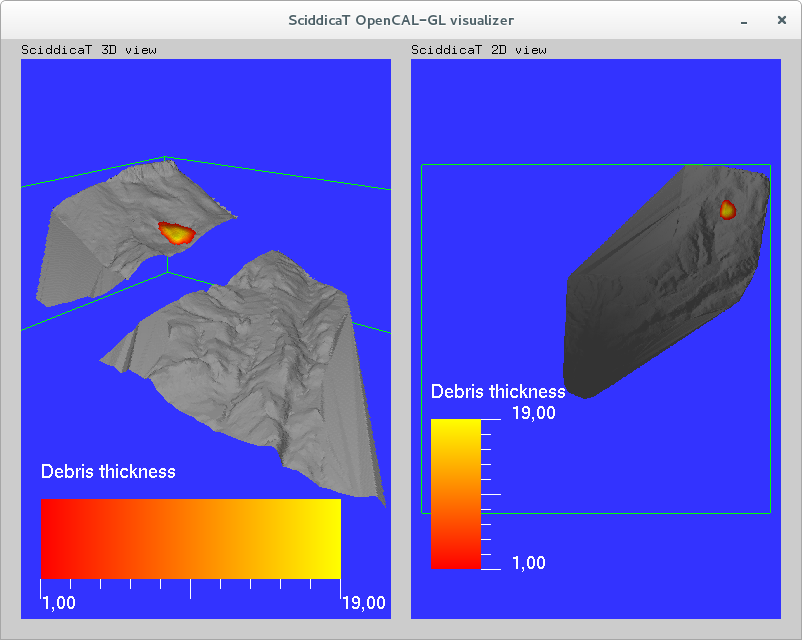
\includegraphics[width=12cm]{./images/OpenCAL/calgl_sciddicaT3}
    \caption{Screenshot of the SciddicaT debris flow model with a
      multi-view 2D and 3D visualization system based on
      OpenCAL-GL. First view is obtained by cutting off some rows and
      columns of the cellular space from representation.}
    \label{fig:calgl_sciddicaT3}
  \end{center}
\end{figure}

Eventually, if you remove the comments at lines 214-216, you will
obtain a partial view for the CA which, for instance, can be used to
represent cross sections. In the specific case of SciddicaT, you will
obtain the result shown in Figure \ref{fig:calgl_sciddicaT3}. Calls at
lines 214-215 only set the column index $j$ to vary from 300 and the
number of columns of the CA model by firstly removing all the indices
form visualization (line 214) and then adding the interval [300,
  \verb'draw_model3D->calModel->columns']. Similarly, line 216 acts on
the row index, $i$, by hiding from visualization the indices
belonging to the interval [100, 150].

\subsection{Implementing the \emph{mod2} CA in OpenCAL and OpenCAL-GL}

As for the previous example about SciddicaT, here we re-propose the
\emph{mod2} CA application to which we added an OpenCAL-GL viewer. The
complete source code is shown in Listing \ref{lst:calgl_mod2} for the
sake of completeness, while Figure \ref{fig:calgl_mod2} shows a
screenshot of the application.

\lstinputlisting[label=lst:calgl_mod2, caption=An OpenCAL
  implementation of the mod2 3D CA with openCAL-GL graphic
  output.]{../opencal-examples/OpenCAL-GL/calgl_mod2CA3D/source/mod2CA.c}

\begin{figure}
  \begin{center}
    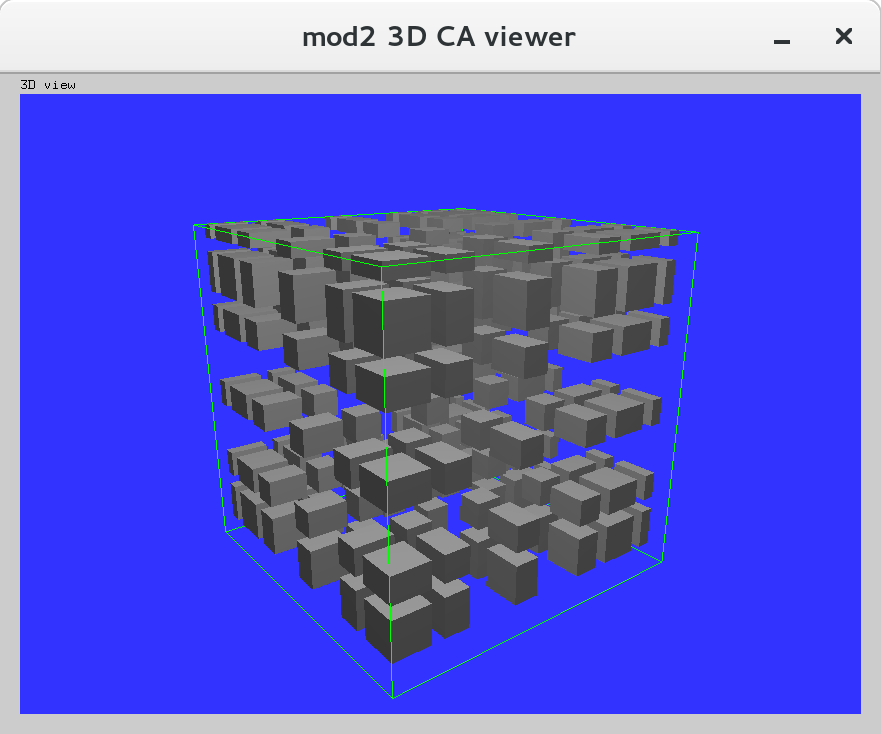
\includegraphics[width=12cm]{./images/OpenCAL/calgl_mod2}
    \caption{Screenshot of the \emph{mod2} 3D CA viewer based on
      OpenCAL-GL.}
    \label{fig:calgl_mod2}
  \end{center}
\end{figure}

As seen, here we consider the 3D implementation of
OpenCAL-GL. In fact, the \verb'OpenCAL-GL/calgl3D.h' and
\verb'OpenCAL-GL/calgl3DWindow.h' headers are included. Moreover, the
OpenCAL-GL functions, already seen in the 2D version in previous
sections, are here in their 3D form (see, e.g., the
\verb'calglAddToDrawModel3Db()' function at line 80). They are
completely equivalents to the 2D versions and therefore they will not
be commented. Eventually, note that statements at lines 86-91 are
commented. If you remove the comments, you will end with some parts of
the cellular space cut down form visualization.


\section{OpenCAL Global Operation Functions}\label{sec:redution}

OpenCAL comes with some functions you can use to perform global
operations over the cellular space, which essentially are reduction
function. Note that such functions should not be used within
elementary processes, but only in the initialization, steering and
stop condition callback functions. The proper use of global functions
is your own responsibility.

In order to use global functions, simply include the
\verb'cal2DReduction.h' header file for 2D CA, or
\verb'cal3DReduction.h' for 3D CA. Table \ref{tab:reductions} lists
the OpenCAL's global reduction functions. All of these functions
accepts a pointer to a CA object and a pointer to a substate over
which execute the global operation as parameters, and return the value
corresponding to the performed reduction. For instance, if you want to
know the maximum value of the substate \verb'Q.h' of the SciddicaT CA,
you can write something like in Listing \ref{lst:reduction_example}.



\begin{table}
  \centering
  \footnotesize
  \begin{tabular}{l|l}
    \hline
    Reduction Functions & Meaning \\
    \hline
    \verb'calReductionComputeMax2Dr()'       & Return the maximum value\\
    \verb'calReductionComputeMin2Dr()'       & Return the minimum value\\
    \verb'calReductionComputeSum2Dr()'       & Return the sum of all substate elements\\
    \verb'calReductionComputeProd2Dr()'      & Return the product of all substate elements\\
    \verb'calReductionComputeLogicalAnd2Dr'  & Return the logical AND of all substate elements\\
    \verb'calReductionComputeBinaryAnd2Dr()' & Return the binary AND of all substate elements\\
    \verb'calReductionComputeLogicalOr2Dr()' & Return the logical OR of all substate elements\\
    \verb'calReductionComputeBinaryOr2Dr()'  & Return the binary OR of all substate elements\\
    \verb'alReductionComputeLogicalXor2Dr()' & Return the logical AND of all substate elements\\
    \verb'calReductionComputeBinaryXor2Dr()' & Return the binary AND of all substate elements\\
    \hline
  \end{tabular}
  \caption{OpenCAL's global reduction functions for 2D CA and
    substates containing floating point values. In order to obtain the
    corresponding functions for 3D CA, you need to change 2D in 3D
    into the functions' suffix, while to obtain the equivalent
    versions for the other supported basic data types, change the last
    suffix character from r to b or i, for CALbyte- or CALint-based
    substates, respectively.}
  \label{tab:reductions}
\end{table}


\begin{lstlisting}[float, label=lst:reduction_example, caption=An example of global reduction operation., numbers=none]
  // ...
  #include <cal2DReduction.h>

  // ...
  void sciddicaTSteering(struct CALModel2D* sciddicaT)
  {
    CALreal max_width;
    max_width = calReductionComputeMax2Dr(sciddicaT, Q.h);
    //...
  }

  // ...
\end{lstlisting}
